\documentclass[a4paper, 12pt]{book}

\usepackage[a4paper, left=2.5cm, right=2.5cm, top=3cm, bottom=3cm]{geometry}
\usepackage{times}
\usepackage{caption}
\usepackage{subcaption}
\usepackage[utf8]{inputenc}
\usepackage{fancyhdr}
\setlength{\headheight}{16pt}
\usepackage{listings}
\usepackage[spanish]{babel} % 
\usepackage{url}
\usepackage{multicol}
\setlength{\columnsep}{1cm}
%\usepackage[dvipdfm]{graphicx}
\usepackage{graphicx}
\usepackage{float}  
\usepackage[nottoc, notlot, notlof, notindex]{tocbibind} 
\usepackage{latexsym}  %% Logo LaTeX
\usepackage{color}
\usepackage{xcolor}
\colorlet{punct}{red!60!black}
\definecolor{lightgray}{rgb}{.9,.9,.9}
\definecolor{darkgray}{rgb}{.4,.4,.4}
\definecolor{purple}{rgb}{0.65, 0.12, 0.82}
\definecolor{background}{HTML}{EEEEEE}
\definecolor{delim}{RGB}{20,105,176}
\colorlet{numb}{magenta!60!black}

\lstdefinelanguage{json}{
    basicstyle=\tiny\ttfamily,
    numbers=left,
   numberstyle=\tiny,
    stepnumber=1,
    numbersep=8pt,
    showstringspaces=false,
    breaklines=true,
    frame=lines,
    backgroundcolor=\color{background},
    literate=
     *{0}{{{\color{numb}0}}}{1}
      {1}{{{\color{numb}1}}}{1}
      {2}{{{\color{numb}2}}}{1}
      {3}{{{\color{numb}3}}}{1}
      {4}{{{\color{numb}4}}}{1}
      {5}{{{\color{numb}5}}}{1}
      {6}{{{\color{numb}6}}}{1}
      {7}{{{\color{numb}7}}}{1}
      {8}{{{\color{numb}8}}}{1}
      {9}{{{\color{numb}9}}}{1}
      {:}{{{\color{punct}{:}}}}{1}
      {,}{{{\color{punct}{,}}}}{1}
      {\{}{{{\color{delim}{\{}}}}{1}
      {\}}{{{\color{delim}{\}}}}}{1}
      {[}{{{\color{delim}{[}}}}{1}
      {]}{{{\color{delim}{]}}}}{1},
}
\lstdefinelanguage{JavaScript}{
  keywords={let,typeof, new, true, false, catch, function, return, null, catch, switch, var, if, in, while, do, else, case, break},
  keywordstyle=\color{blue}\bfseries,
  ndkeywords={class, export, boolean, throw, implements, import, this},
  ndkeywordstyle=\color{darkgray}\bfseries,
  identifierstyle=\color{black},
  sensitive=false,
  comment=[l]{//},
  morecomment=[s]{/*}{*/},
  commentstyle=\color{purple}\ttfamily,
  stringstyle=\color{red}\ttfamily,
  morestring=[b]',
  morestring=[b]"
}

\lstdefinelanguage{CSS}{
  morekeywords={accelerator,azimuth,background,background-attachment,
    background-color,background-image,background-position,
    background-position-x,background-position-y,background-repeat,
    behavior,border,border-bottom,border-bottom-color,
    border-bottom-style,border-bottom-width,border-collapse,
    border-color,border-left,border-left-color,border-left-style,
    border-left-width,border-right,border-right-color,
    border-right-style,border-right-width,border-spacing,
    border-style,border-top,border-top-color,border-top-style,
    border-top-width,border-width,bottom,caption-side,clear,
    clip,color,content,counter-increment,counter-reset,cue,
    cue-after,cue-before,cursor,direction,display,elevation,
    empty-cells,filter,float,font,font-family,font-size,
    font-size-adjust,font-stretch,font-style,font-variant,
    font-weight,height,ime-mode,include-source,
    layer-background-color,layer-background-image,layout-flow,
    layout-grid,layout-grid-char,layout-grid-char-spacing,
    layout-grid-line,layout-grid-mode,layout-grid-type,left,
    letter-spacing,line-break,line-height,list-style,
    list-style-image,list-style-position,list-style-type,margin,
    margin-bottom,margin-left,margin-right,margin-top,
    marker-offset,marks,max-height,max-width,min-height,
    min-width,-moz-binding,-moz-border-radius,
    -moz-border-radius-topleft,-moz-border-radius-topright,
    -moz-border-radius-bottomright,-moz-border-radius-bottomleft,
    -moz-border-top-colors,-moz-border-right-colors,
    -moz-border-bottom-colors,-moz-border-left-colors,-moz-opacity,
    -moz-outline,-moz-outline-color,-moz-outline-style,
    -moz-outline-width,-moz-user-focus,-moz-user-input,
    -moz-user-modify,-moz-user-select,orphans,outline,
    outline-color,outline-style,outline-width,overflow,
    overflow-X,overflow-Y,padding,padding-bottom,padding-left,
    padding-right,padding-top,page,page-break-after,
    page-break-before,page-break-inside,pause,pause-after,
    pause-before,pitch,pitch-range,play-during,position,quotes,
    -replace,richness,right,ruby-align,ruby-overhang,
    ruby-position,-set-link-source,size,speak,speak-header,
    speak-numeral,speak-punctuation,speech-rate,stress,
    scrollbar-arrow-color,scrollbar-base-color,
    scrollbar-dark-shadow-color,scrollbar-face-color,
    scrollbar-highlight-color,scrollbar-shadow-color,
    scrollbar-3d-light-color,scrollbar-track-color,table-layout,
    text-align,text-align-last,text-decoration,text-indent,
    text-justify,text-overflow,text-shadow,text-transform,
    text-autospace,text-kashida-space,text-underline-position,top,
    unicode-bidi,-use-link-source,vertical-align,visibility,
    voice-family,volume,white-space,widows,width,word-break,
    word-spacing,word-wrap,writing-mode,z-index,zoom},
  morestring=[s]{:}{;},
  sensitive,
  morecomment=[s]{/*}{*/}
}
\lstset{
   language=JavaScript,
   backgroundcolor=\color{background},
   extendedchars=true,
   basicstyle=\tiny\ttfamily,
   showstringspaces=false,
   showspaces=false,
   numbers=left,
   numberstyle=\tiny,
   numbersep=9pt,
   tabsize=1,
   breaklines=true,
   showtabs=false,
   captionpos=b
}

\title{Memoria del Proyecto}
\author{Rubén Álvarez Martín}

\renewcommand{\baselinestretch}{1.5}  
\renewcommand{\appendixname}{Apéndice}

\begin{document}

% PORTADA
\begin{titlepage}
\begin{center}
\begin{tabular}[c]{c c}
%
\includegraphics[bb=0 0 194 352, scale=0.25]{logo} &

\includegraphics[scale=0.25]{img/logo_vect.png} &
\begin{tabular}[b]{l}
\Huge
\textsf{UNIVERSIDAD} \\
\Huge
\textsf{REY JUAN CARLOS} \\
\end{tabular}
\\
\end{tabular}

\vspace{3cm}

\Large
GRADO EN INGENIERÍA TELEMÁTICA
\vspace{0.4cm}

\large
Curso Académico 2019/2020

\vspace{0.8cm}

Trabajo Fin de Grado

\vspace{2.5cm}

\LARGE
Mejoras en entorno de robótica educativa para niños \vspace{4cm}

\large
Autor : Rubén Álvarez Martín \\
Tutor : Dr. José María Cañas Plaza \\
\end{center}
\end{titlepage}

\newpage
\mbox{}
\thispagestyle{empty} 

% RESUMEN %
%%%%%%%%%%%%%%%%%%%%%%%%%%%%%%%%%%%%%%%%%%%

\chapter*{Resumen}
\markboth{RESUMEN}{RESUMEN} 

     Este proyecto está muy relacionado con las tecnologías web y la robótica y está enfocado a la mejora de la plataforma \emph{Kibotics} en la cual se dispone de un simulador robótico que tiene todo su peso computacional en el navegador web. Esta plataforma está enfocada a enseñar robótica y programación a estudiantes desde muy corta edad hasta estudiantes de secundaria, empleando el lenguaje \emph{Scratch} en cortas edades y \emph{Python} en más avanzadas. Con ella, además de ejecutar el código programado, se puede enviar el mismo a un robot físico haciendo la traducción a \emph{Python}. \\
    
    
    Como aportes genuinos de este TFG se han añadido a \textit{Kibotics} soporte a nuevos robots tales como drones o mBot, nuevos ejercicios a partir de la funcionalidad existente y ejercicios competitivos que permiten programar dos \textit{robots} en el mismo escenario y que compitan entre sí. Estos ejercicios incorporan evaluadores automáticos que evaluan el comportamiento de los \textit{robots} simulados y con ello la eficacia del código del estudiante. Además se ha desarrollado una página web para poder teleoperar los robots sin necesidad de programarlos y comprobar sus sensores y actuadores. \\
    
    
    Para el desarrollo de software de todas las mejoras se han empleado herramientas como \textit{A-Frame}, \textit{HTML5}, \textit{JavaScript}, \textit{Blender} o \textit{Blockly}. Para la gestión de dependencias del proyecto se utiliza NPM y para el empaquetado de la aplicación, WebPack.

%%%%%%%%%%%%%%%%%%%%%%%%%%%%%%%%%%%%%%%%%%%%%%%%%%%%%%%%%%%%%%%%%%%%%%%%%%%%%%%%
% ÍNDICES %

%%%% Índice de contenidos
\tableofcontents
%%%% Índice de figuras
\cleardoublepage
\addcontentsline{toc}{chapter}{Lista de figuras} % para que aparezca en el indice de contenidos
\listoffigures % indice de figuras
%%%% Índice de tablas
\cleardoublepage
\addcontentsline{toc}{chapter}{Lista de tablas} % para que aparezca en el indice de contenidos
\listoftables % indice de tablas
%%%%%%%%%%%%%%%%%%%%%%%%%%%%%%%%%%%%%%%%%%%%%%%%%%%%%%%%%%%%%%%%%%%%%%%%%%%%%%%%

\cleardoublepage
\pagestyle{fancy}
\setlength{\parindent}{6mm}
\pagenumbering{arabic} 

% INTRODUCCIÓN %
%%%%%%%%%%%%%%%%%%%%%%%%%%%%%%%%%%%%%%%%%%%%%%%%%%%%%%%%%%%%%%%%%%%%%%%%%%%%%%%%


\chapter{Introducción}
\label{chap:intro} 
El principal objetivo del proyecto es mejorar la plataforma \textit{Websim} para disponer de más robots y ejercicios para incrementar su valor educativo dando más posibilidades de aprendizaje. 
   
 \section{Tecnologías web}
\label{sec:web}
Las tecnologías web han ido evolucionando a los largo de la historia, pero todas se basan en un modelo cliente-servidor. Para lograr la comunicación entre cliente y servidor, se necesita un navegador por parte del cliente y un servidor web capaz de atender las solicitudes. El protocolo que es utilizado para esta comunicación se llama \textit{HTTP}.
\subsection{HTTP}
\label{subsec:http}

\subsection{Tecnologías en servidor}
\label{subsec:tecserver}

\subsection{Tecnologías en cliente}
\label{subsec:tecclient}


\section{Robótica}
\label{sec:robotica}
La robótica es una rama tecnológica encargada del diseño y construcción de aparatos que realizan operaciones y trabajos en sustitución de la mano de obra humana. 

Un robot es un sistema autónomo programable capaz de realizar tareas de ayuda al ser humano y con aplicaciones en campos diversos como medicina, hogar, fábricas, etc. 

Los robots se componen de sensores, controladores y actuadores.
\begin{itemize}
    \item Sensores: son los encargados de recoger información del entorno. En este grupo se encuentran láser, cámaras, ultrasonidos u odómetros. Estos dispositivos equivalen a los sentidos humanos. 
    \item Controladores: analizan los datos recogidos por los sensores y elaboran una respuesta que va a ser enviada a los actuadores. En los seres humanos equivale al cerebro. 
    \item Actuadores: se encargan de transformar energía eléctrica, hidráulica o neumática en mecánica. Son los interactúan con el entorno y equivalen a los músculos humanos. 
\end{itemize}

\subsection{Historia}
La palabra robot fue empleada por primera vez en 1920 por Karel Capek, un escritor checo que realiza una obra de teatro en la que un hombre fabrica un robot. 

Años más tarde, en 1950, Isaac Asimov publica un libro llamado \textit{Yo, Robot} en el que acuña la palabra robótica definiendo a la ciencia que estudia a los robots. En el también se incluyen tres leyes de la robótica:
\begin{itemize}
    \item Un robot no hará daño a un ser humano ni permitirá que un ser humano sufra ningún tipo daño.
    \item Un robot debe cumplir las órdenes recibidas por un ser humano, salvo las que entren en conflicto con la primera ley.
    \item Un robot debe proteger su propia existencia mientras que no entre en conflicto con ninguna de las leyes anteriores. 
\end{itemize}{}

Es a finales de la década de los 50 cuando la robótica sufre el mayor impulso al crearse el primer robot comercial en 1956 y, años más tarde, en 1961, se instala el primer robot industrial (Figura \ref{fig:unimate}).  

\begin{figure}[H]
\centering
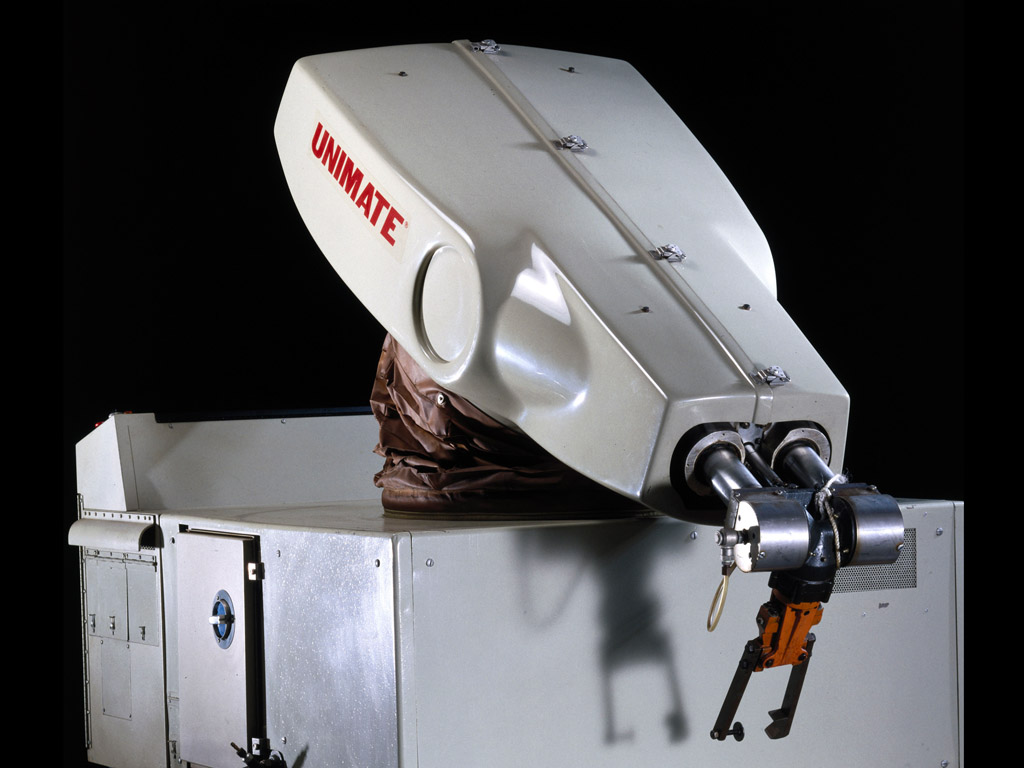
\includegraphics[scale=0.2]{img/unimate.jpg}
\caption{Unimate, primer robot industrial} \label{fig:unimate}
\end{figure}

En los años 70 se crea el primer robot autónomo, \textit{Shakey}  (Figura \ref{fig:shakey}). Fue el primero que incorporaba inteligencia artificial y disponía de control de motores y sensores. \textit{Shakey} era capaz de recoger toda la información de su entorno, crear un mapa y diseñar el camino más corto desde su ubicación al destino. 


\begin{figure}[H]
\centering
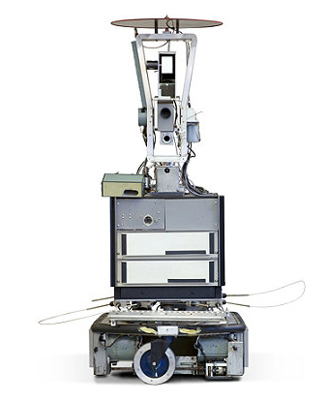
\includegraphics[width=0.5\textwidth]{img/shakey.jpg}
\caption{Shakey, primer robot autónomo} \label{fig:shakey}
\end{figure}

En 2000 la compañía Honda lanza el robot \textit{Asimo} (Figura \ref{fig:asimo}), un robot humanoide capaz de detectar múltiples objetos, reconocer caras e interpretar comandos de voz o gestos.\textit{Asimo} fue creado con el objetivo de, algún día, ofrecer asistencia a personas con necesidades especiales. 

\begin{figure}[H]
\centering
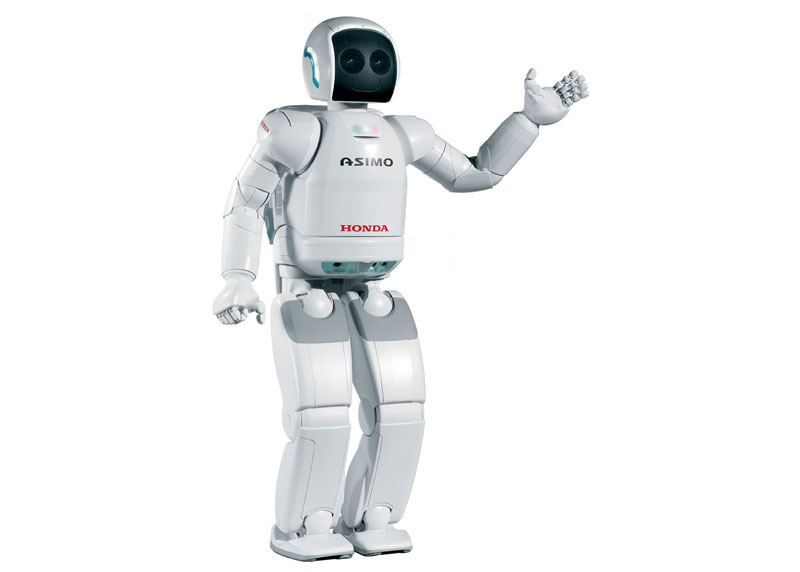
\includegraphics[width=0.5\textwidth]{img/asimo-honda.jpg}
\caption{Asimo, primer robot humanoide} \label{fig:asimo}
\end{figure}

Es en 2011 cuando la robótica alcanza uno de sus mayores hitos gracias al robot explorador \textit{Curiosity} (Figura \ref{fig:curiosity}). Este robot llego a Marte en 2012 y su cometido fue investigar el planeta para determinar si existió vida en Marte, caracterizar su clima y geología y preparar el entorno para su exploración humana. 

\begin{figure}[H]
\centering
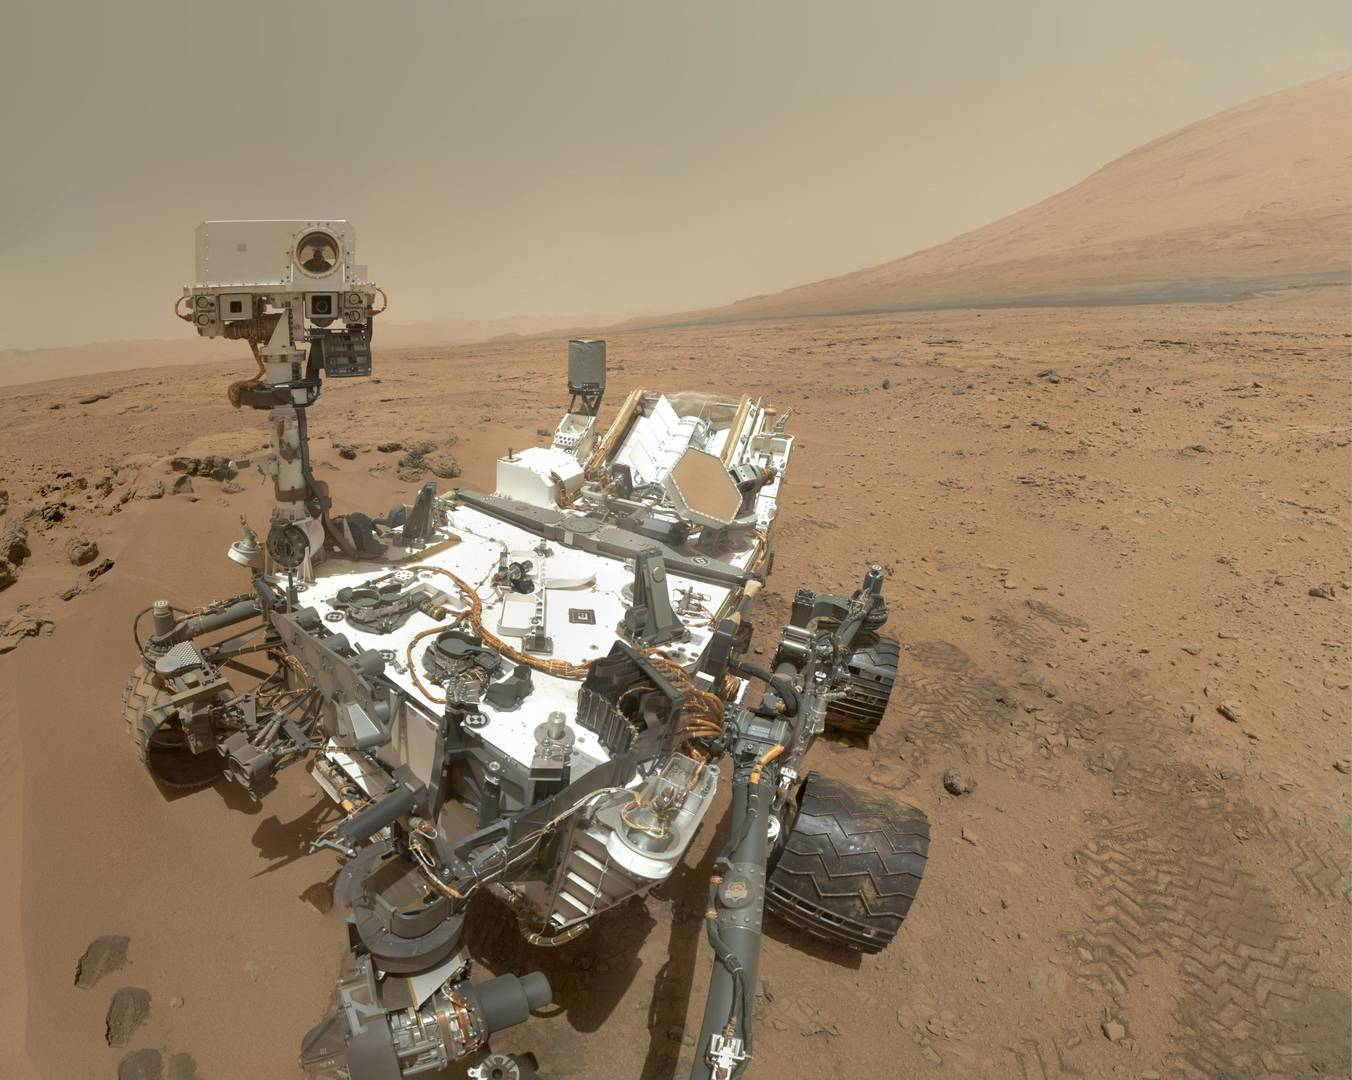
\includegraphics[width=0.8\textwidth]{img/curiosity.jpg}
\caption{Autorretrato del Curiosity en Marte} \label{fig:curiosity}
\end{figure}


Hoy en día no solo se ven robots en entornos industriales, si no que aparecen cada vez más en entornos domésticos, educativos o automovilístico.

\subsection{Tipos de robots}
\label{subsec:tiposRobots}


\section{Robótica educativa}
\label{sec:educativa}

\chapter{Objetivos}
\label{chap:objetives}
\section{Objetivos}
\section{Metodología}


% OBJETIVOS %
%%%%%%%%%%%%%%%%%%%%%%%%%%%%%%%%%%%%%%%%%%%%%%%%%%%%%%%%%%%%%%%%%%%%%%%%%%%%%%%%
\chapter{Objetivos y metodología}
Una vez expuestas las motivaciones y contexto del proyecto, en este capítulo se detallarán objetivos y metodología empleada. 

\label{chap:objetivos}
\section{Objetivos}
El propósito de este proyecto es la extensión y mejora de una herramienta docente para facilitar el aprendizaje de algoritmos y robótica. Para cumplir ese propósito se han fijado varios objetivos:
\begin{itemize}
    \item Añadir soporte para \textit{drone} en la plataforma, incluyendo tanto el software necesario como el modelo 3D para el entorno de \textit{A-Frame}.
    
    \item Incluir más ejercicios a \textit{WebSim}. Es necesario elaborar archivos de configuración para poder cambiar entre los distintos ejercicios y robots soportados. Esto incluye añadir más modelos de robots y nuevos escenarios a la plataforma.
    
    \item Añadir teleoperadores para que se puedan controlar los robots sin necesidad de programar. De esta manera se facilita la labor de los desarrolladores al poderse probar el entorno y los sensores del robot de manera sencilla.
    
    \item Incluir ejercicios competitivos de tal manera que dos usuarios puedan programar sobre el mismo escenario. Este objetivo también incluye crear un evaluador para puntuar el comportamiento de cada robot. 
    
\end{itemize}
\section{Metodología}
\label{sec:metodologia}



\section{GitHub}
\label{sec:github}

% HERRAMIENTAS %
%%%%%%%%%%%%%%%%%%%%%%%%%%%%%%%%%%%%%%%%%%%%%%%%%%%%%%%%%%%%%%%%%%%%%%%%%%%%%%%%
\chapter{Herramientas}
\label{chap:herramientas}
En este capítulo se van a detallar las herramientas utilizadas en el desarrollo de este proyecto. Algunas se han elegido por facilidad de uso y otras por necesidad del entorno desarrollado.

% JAVASCRIPT %
\section{JavaScript}
\label{sec:js}
\textit{JavaScript} es un lenguaje interpretado de alto nivel que se encuentra bajo el estándar \textit{ECMAScript}\footnote{Especificación de lenguaje de programación el cual define tipos dinámicos y soporta características de programación orientada a objetos.} y está basado en otros lenguajes de programación como Java o C. 

En su principio fue concebido como lenguaje para el lado cliente, implementado en un navegador web, permitiendo mejorar la interfaz de usuario y realizar páginas web dinámicas.

En la actualidad, JavaScript se ha ido extendiendo hacia el lado servidor y es por ello que es el lenguaje más utilizado para desarrollo web y todos los navegadores interpretan el código integrado en las páginas web.
\subsection{Características}
Las siguientes características tienen en común que todas se ajustan al estándar de ECMAScript: 
\begin{itemize}
    \item Es un lenguaje estructurado, tiene gran similitud con \textit{C} y comparte gran parte de su estructura (bucles, condicionales, sentencias...) a excepción del alcance de sus variables. En \textit{C} su ámbito es el bloque en el que fue definida y, en su origen, \textit{JavaScript} tenía un alcance global en las variables definidas. Es en ECMAScript 2015 cuando se añade la palabra clave \textit{let}, que incorpora compatibilidad con \textit{block scoping} (alcance de la variable en el bloque en la que es definida). 
    \item Tipado débil, por el cual el tipo de datos está asociado al valor, no a la variable. Esto significa que una variable puede ser \textit{number} o \textit{string} en distintos momentos de ejecución. 
    \item Formado en su totalidad por objetos, en los cuales los nombres de sus propiedades son claves de tipo cadena siendo \textit{objeto.a = 1} y \textit{objeto['a'] = 1} equivalentes. 
    \item Lenguaje interpretado, es por esto que no requiere un compilador ni crear un fichero binario del código; cada navegador tiene su intérprete que se encarga de ejecutarlo.
    \item Evaluación en tiempo de ejecución gracias a la función \textit{eval}, la cual evalúa un código en \textit{JavaScript} representado como una cadena de caracteres. 

    
\end{itemize}
% A-FRAME %
\section{A-Frame}
\label{sec:aframe}
A-Frame es un framework de código abierto destinado a crear experiencias de realidad virtual a partir de \textit{HTML} de forma que sea sencillo de leer y comprender. De esta manera es accesible para crear una gran comunidad. 


Además tiene compatibilidad con \textit{Vive}, \textit{Rift}, \textit{Windows Mixed Reality}, \textit{Daydream}, \textit{GearVR} y \textit{CardBoard} así como soporte para todos los controladores respectivos. También ofrece soporte para ordenadores de escritorio y para la mayoría de teléfonos inteligentes.

\subsection{HTML y primitivas}
\textit{A-Frame }se basa en \textit{HTML} y el \textit{DOM} usando un \textit{polyfill}\footnote{Fragmento de código en \textit{JavaScript} utilizado para proporcionar una funcionalidad moderna en navegadores antiguos.} para elementos personalizados. \textit{HTML} es un componente básico para Web y como tal, tiene una gran accesibilidad como lenguaje. Para crear una escena de realidad virtual con \textit{A-Frame} no se requiere ninguna instalación y simplemente con la creación del \textit{HTML} se puede abrir en el navegador. La mayoría de herramientas existentes(como \textit{React}, \textit{Vue.js}, \textit{d3.js} y \textit{jQuery}) funcionan en este framework. 

\textit{HTML} y \textit{DOM} son solo la capa más externa del framework, debajo se encuentra el componente \textit{three.js} en el que está basado \textit{A-Frame} gracias al cual un componente puede ser utilizado en distintas entidades. De esta manera hace posible seguir el principio de programación \textit{Don't Repeat Yourself} ya que, una vez registrada una primitiva, se puede hacer referencia al elemento todas las veces que sea necesario.  

A-Frame proporciona elementos como \textit{a-box} o \textit{a-sky} llamados primitivas. Podemos crear un escenario a través de estas primitivas como el mostrado en la figura \ref{fig:scene1} con el siguiente código: 

\begin{lstlisting}[language=javascript, caption=Código con primitivas que representa un escenario]
<!DOCTYPE html>
<html>
  <head>
    <meta charset="utf-8">
    <title>Escenario primitivas</title>
    <script src="https://aframe.io/releases/0.9.2/aframe.min.js"></script>
  </head>
  <body>
    <a-scene background="color: #FAFAFA">
      <a-box position="-1 0.5 -3" rotation="0 45 0" color="#4CC3D9" shadow></a-box>
      <a-sphere position="0 1.25 -5" radius="1.25" color="#ff0000" shadow></a-sphere>
      <a-cylinder position="1 0.75 -3" radius="0.5" height="1.5" color="#FFC65D" shadow></a-cylinder>
      <a-plane position="0 0 -4" rotation="-90 0 0" width="4" height="4" color=" #1cde83" shadow></a-plane>
      <a-sky color="#e7e1e0"></a-sky>
    </a-scene>
  </body>
</html>
\end{lstlisting}

\begin{figure}[H]
\centering
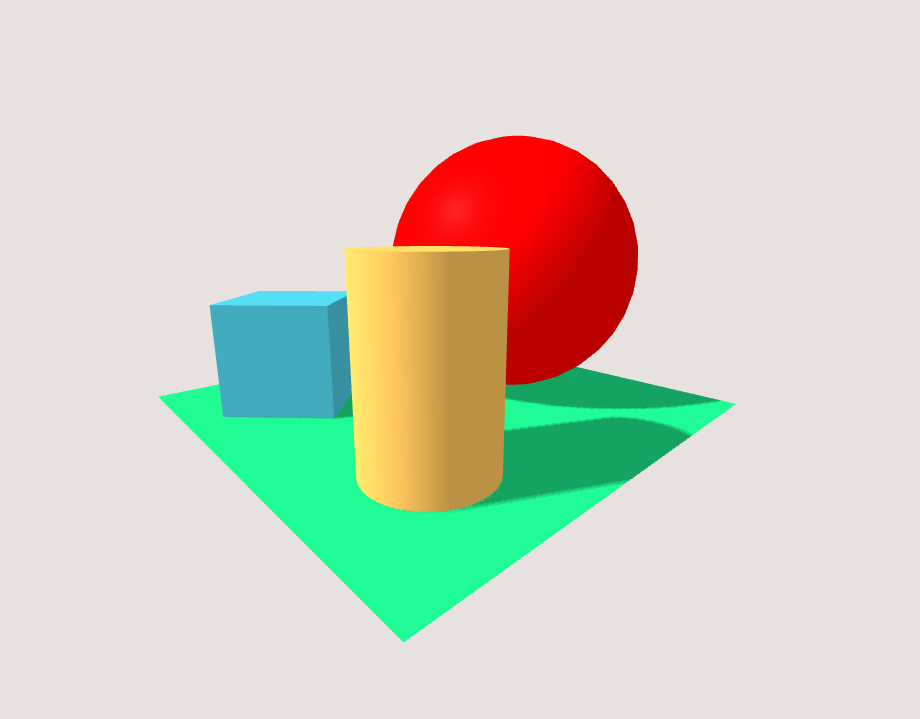
\includegraphics[width=0.8\textwidth]{img/scene1.png}
\caption{Escenario a-frame} \label{fig:scene1}
\end{figure}

A-Frame, además de disponer primitivas como las mostradas, hace posible la creación de primitivas para poder elaborar escenas lo más completas posible. También se pueden incluir entidades más complejas a partir de modelos 3D en formatos como \textit{gltf}, \textit{obj} o \textit{collada} de los cuales se hablará en siguientes apartados.

\subsection{Entidad, Componente y Sistema}

    Como ya se ha comentado, A-Frame es un framework \textit{three.js} con una arquitectura de entidad-componente-sistema (\textit{ECS}). Es un patrón común en 3D y desarrollo de juegos que siguen la composición sobre el principio de herencia y jerarquía. Algunos beneficios que \textit{ECS} aporta son mayor flexibilidad al definir objetos, gran escalabilidad o eliminación de problemas de largas cadenas de herencia. Existe un \textit{API} que representa cada pieza de \textit{ECS}: 
    \begin{itemize}
    \item Una entidad se representa con la etiqueta \textit{a-entity}. 
        \begin{lstlisting}[language=HTML]
        <a-entity geometry="primitive: box" material="color: red">
        \end{lstlisting}
        En este ejemplo se hace uso de \textit{a-entity} para crear una caja de color rojo. 

    
    \item Un componente se representa como un atributo de HTML. Cada componente es un objeto que tiene un esquema, manejadores y métodos. Para registrar componentes se utiliza el método de A-Frame \textit{registerComponent}.
    
    \begin{lstlisting}[language=javascript, caption=Código para registrar un componente]
        AFRAME.registerComponent('example', {
          init: function () {
            var el = this.el;
            el.setObject3D('mesh', new THREE.Mesh());
            el.getObject3D('mesh');  // Returns THREE.Mesh that was just created.
          }
        });
    \end{lstlisting}
    
    \item Un sistema es el representado por atributos HTML mediante la etiqueta \textit{a-scene}. Se registran de manera similar a un componente; gracias al método \textit{registerSystem}.
\end{itemize}


% BLOCKLY %
\section{Blockly}
\label{sec:blockly}
\textit{Blockly} es una librería que añade un editor de código visual a aplicaciones web y móviles. Utiliza bloques gráficos para representar conceptos complejos de código de manera más sencilla. De esta manera permite a los usuarios aplicar  principios de programación sin tener que preocuparse por la sintaxis y ayuda a iniciarse y a aprender a programar a estudiantes de temprana edad. Esta librería está diseñada por las personas que están detrás de \textit{Scratch}\footnote{\url{https://scratch.mit.edu/}} del MIT y construido sobre su base de código. 

\subsection{Traductor de código}
\textit{Blockly} es para desarrolladores y las \textit{aplicaciones Blockly} son pensadas para estudiantes. Desde la perspectiva de usuario, \textit{Blockly} es una forma visual e intuitiva de crear código y, desde la de desarrollador, es una interfaz de usuario preparada para crear un lenguaje visual que emite código y se puede exportar a otros lenguajes de programación como \textit{JavaScript}, \textit{Python}, \textit{PHP}, \textit{Lua} o \textit{Dart}. 

Estos generadores de código aportan las herramientas para crear funciones, condicionales, bucles, etc. El principal problema de esto es que en ocasiones se requiere del uso de APIs de otras dependencias. \textit{Blockly} aporta una solución; un generador de bloques personalizados que traduce al código que deseemos. Esto aporta mucha flexibilidad y da la funcionalidad deseada para el desarrollo de este proyecto. 

\subsection{Bloques personalizados}
Como se ha explicado, \textit{Blockly} dispone de una gran cantidad de bloques predefinidos; desde funciones matemáticas hasta estructuras en bucle. Sin embargo, para interactuar con una aplicación externa, se deben crear bloques personalizados para formar una API. Según la documentación ofrecida por \textit{Google}\footnote{\url{https://developers.google.com/blockly/guides/create-custom-blocks/overview}}, la mejor forma de crear un bloque es buscar un bloque existente con una funcionalidad similar y modificarlo según se necesite. De otra manera, para generar un bloque personalizado, hay varios aspectos a tener en cuenta: 

\begin{itemize}
    \item Primero se define el bloque para determinar su aspecto gráfico y su comportamiento. Esto incluye el texto, color, forma o cómo conectarlos con otros bloques. La configuración de estos parámetros se puede realizar mediante \textit{JSON} o \textit{JavaScript}. El bloque mostrado en la figura \ref{fig:customblock} se puede configurar con los dos métodos de la siguiente manera:
    
    %definir JSON como lenguaje
     \begin{lstlisting}[language=json, caption=Código en JSON para configurar un bloque personalizado]
     {
      "type": "block_test",
      "message0": "%1 %2",
      "args0": [
        {
          "type": "field_label_serializable",
          "name": "NAME",
          "text": "custom_block"
        },
        {
          "type": "input_value",
          "name": "NAME",
          "check": "Number"
        }
      ],
      "inputsInline": false,
      "previousStatement": null,
      "nextStatement": null,
      "colour": 120,
      "tooltip": "This is a custom block",
      "helpUrl": ""
    }
    \end{lstlisting}

    \begin{lstlisting}[language=javascript, caption=Código en javascript para configurar un bloque personalizado]
    Blockly.Blocks['block_test'] = {
      init: function() {
        this.appendValueInput("NAME")
            .setCheck("Number")
            .appendField(new Blockly.FieldLabelSerializable("custom_block"), "NAME");
        this.setInputsInline(false);
        this.setPreviousStatement(true, null);
        this.setNextStatement(true, null);
        this.setColour(120);
     this.setTooltip("This is a custom block");
     this.setHelpUrl("");
      }
    };
    \end{lstlisting}

    \begin{figure}[H]
    \centering
    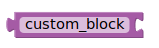
\includegraphics[width=0.2\textwidth]{img/CustomBlock.png}
    \caption{Bloque personalizado} \label{fig:customblock}
    \end{figure}

    \item Configurar la traducción del bloque a la instrucción deseada en los distintos lenguajes necesarios.
    
    \item Inicializar el bloque para que sea visible en el editor visual de código. 
    
    Aunque los parámetros del \textit{JSON} son auto-descriptivos, es complicado generar un bloque desde cero. Es por ello que \textit{Google} facilita  una herramienta de creación de bloques, la cual se muestra en la figura \ref{fig:googleTool}. 
    En ella se puede personalizar todos los aspectos del bloque: texto, color, variables de entrada, formas de conexión con otros bloques, etc.
    Además, permite exportar la configuración del bloque en formato \textit{JSON} o \textit{JavaScript} y muestra una función con la configuración básica para obtener el código en JavaScript(y permite seleccionar el lenguaje deseado entre los admitidos por \textit{Blockly}).
    %% poner nombre a figura
    \begin{figure}[H]
    \centering
    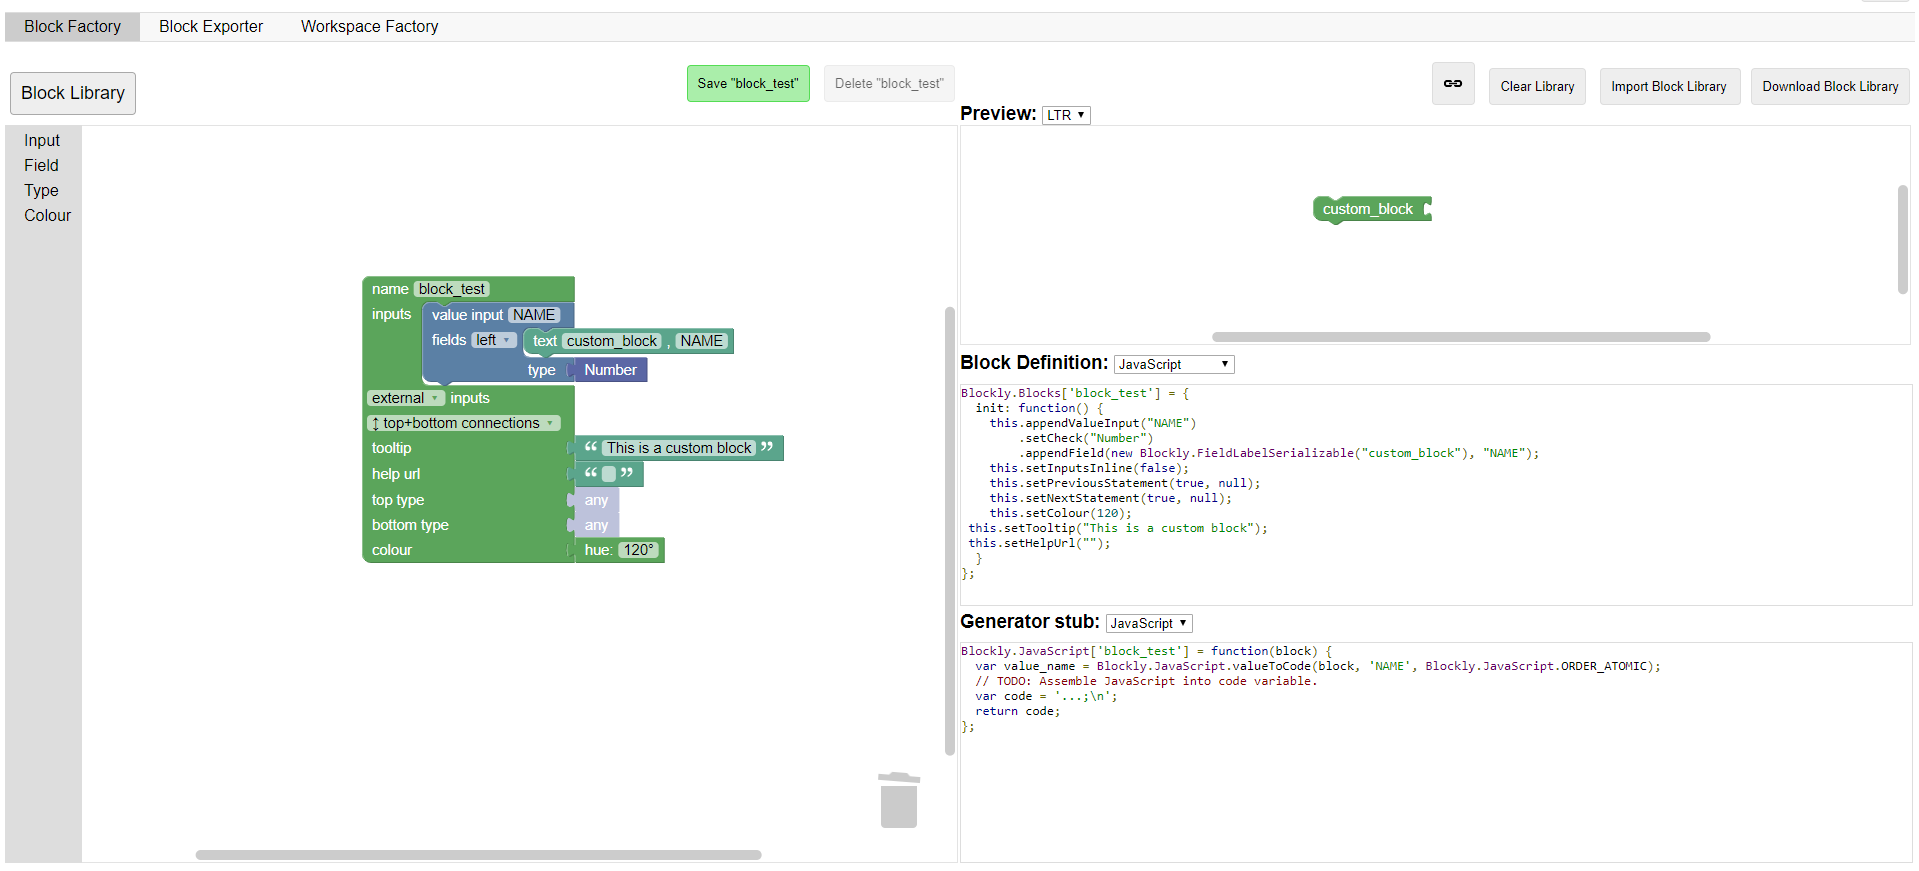
\includegraphics[width=1.1\textwidth]{img/GoogleTool.png}
    \caption{Herramienta para creación de bloques personalizados} \label{fig:googleTool}
    \end{figure}
    
\end{itemize}

% GESTORES DE PAQUETES %
\section{Gestores de paquetes}
\label{sec:gest}
Un gestor de paquetes es una herramienta para automatizar el proceso de instalación, actualización, configuración y eliminación de software. En este proyecto se han utilizado \textit{NPM} y \textit{Webpack} 
\subsection{NPM}
\textit{Node Package Manager} (\textit{NPM}) es el sistema de gestión de dependencias por defecto para \textit{Node.js}, que es un entorno de ejecución para \textit{JavaScript} y permite, con la configuración de un fichero, descargar dependencias y paquetes necesarios para el correcto funcionamiento de la aplicación. Todo ello ha de estar definido en un fichero llamado \textit{package.json} que debe ser escrito en \textit{JSON}. Para usar \textit{NPM} como instalador de paquetes únicamente hay que ejecutar \textit{npm install} en el directorio en el que se encuentre el fichero \textit{package.json}. Además, gracias a este gestor, podemos configurar pequeños \textit{scripts} para ejecutar algún proceso como lanzar una aplicación después de la instalación o empaquetar la aplicación en \textit{bundles} combinándolo con \textit{Webpack}.

\subsection{Webpack}
%https://webpack.js.org/
\textit{Webpack} es un sistema de \textit{bundling} usado para empaquetar una aplicación web en su fase de producción. Se puede considerar una evolución de \textit{Grunt}\footnote{https://gruntjs.com/} y \textit{Gulp}\footnote{https://gulpjs.com/} porque permite automatizar procesos principales tales como transpilar y preprocesar código. 

% BLENDER %
\section{Blender}
\label{sec:blender}

\textit{Blender} es un programa libre dedicado al diseño y animación 3D. Mediante una interfaz gráfica permite diseñar objetos, personajes y escenas en tres dimensiones con muy diversas técnicas. Cada uno de los elementos creados pueden ser animados mediante \textit{keyframing} o animación por fotogramas clave. En su origen \textit{Blender} fue distribuido como una herramienta privada explotada por un estudio de animación, pero actualmente se encuentra bajo licencia \textit{GPL}\footnote{https://www.gnu.org/licenses/gpl-3.0.en.html}. 

Entre las muchas características que ofrece \textit{Blender}, las más útiles para el desarrollo del proyecto son:
\begin{itemize}
    \item Modelados: es el proceso mediante el cual se crean objetos en un espacio 3D de manera digital. Están compuestos de líneas, puntos, cuadrados, triángulos, etc. 
    
    \item Iluminación: existen varios tipos de luz que se pueden adaptar a la escena. Es posible aplicar a cada uno de los objetos para especificar la luz recibida por cada uno de ellos además de variar aspectos como la intensidad, el color o la posición en el escenario.
    
    \item Tracking: permite especificar el comportamiento y características de un determinado objeto en el escenario tridimensional. 
    \item Animaciones: cada objeto se puede animar de manera independiente. Se realiza mediante un \textit{timelapse} en la cual cada posición del \textit{timeline} es un frame en el cual se especifica cualquier tipo de característica (rotación, movimiento, cambio de color, etc).  
    
    \item Texturizado: son un medio para agregar o eliminar detalles a la superficie de un determinado objeto. Proyectando imágenes sobre la superficie del mallado se pueden aplicar patrones para personalizar el aspecto de la textura. 

    Además permite exportar los modelos a los formatos más usados para \textit{A-Frame}: \textit{glTF} y \textit{COLLADA}. 
\end{itemize}
\subsection{COLLADA}
\textit{COLLaborative Design Activity} (\textit{COLLADA}) es un  formato de archivo de intercambio para aplicaciones 3D interactivas. Se define como un esquema \textit{XML} para intercambiar activos digitales entre varias aplicaciones de software de gráficos. Son definidos con la extensión \textit{.dae} y pueden hacer referencia a archivos de imagen adicionales que actúan como texturas del objeto 3D. 

\subsection{glTF}
GL Transmission Format (\textit{glTF}) es una especificación basada en el estándar \textit{JSON} para transmisión y carga eficiente de escenas y modelos 3D para aplicaciones. Este formato minimiza el tamaño de los ficheros y su tiempo de ejecución necesario para desempaquetar y usarlos. Permite animación de los objetos que puede ser activada por \textit{A-Frame} vía \textit{HTML} o dinámicamente con \textit{javaScript}. 
En la figura \ref{fig:tree} se puede ver la figura añadida a un escenario de A-Frame via \textit{HTML}:

\begin{lstlisting}[language=html, caption=Código para añadir un modelo 3D personalizado a A-Frame]
 <a-asset-item id="tree" src="assets/models/CartoonTree.dae"></a-asset-item>
  <a-entity id="a-tree" collada-model="#tree" rotation="0 0 0" position="2.75 0.01 -2.27">
  
\end{lstlisting}

\begin{figure}[H]
\centering
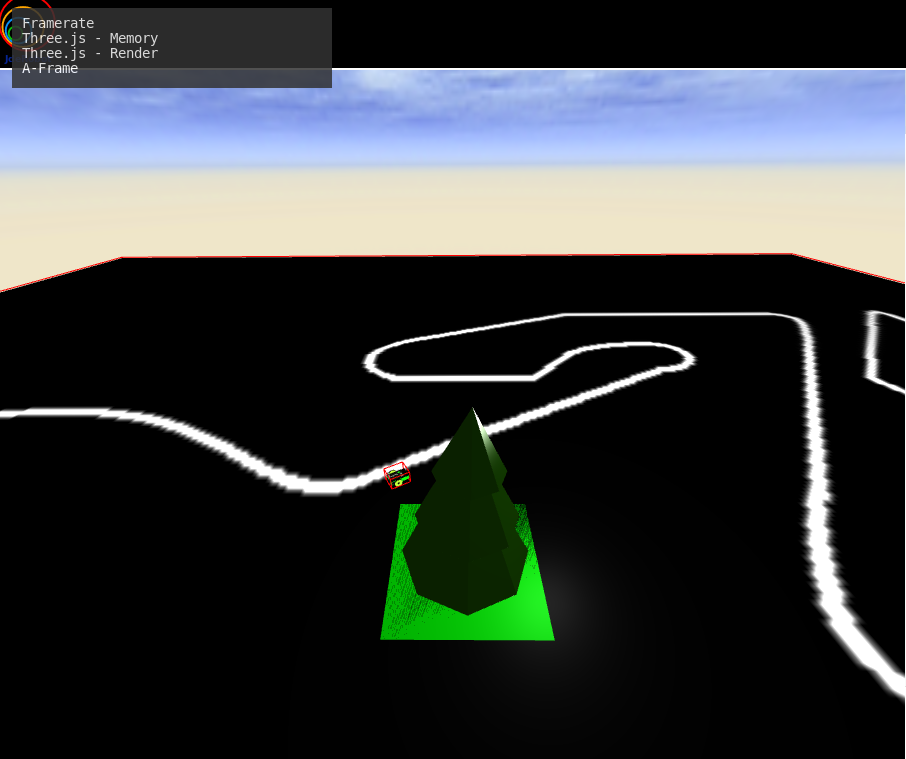
\includegraphics[width=0.8\textwidth]{img/tree_aframe.png}
\caption{Modelo glTF añadido en un escenario de A-Frame} \label{fig:tree}
\end{figure}
Además del \textit{software} explicado en esta sección, existen multitud de herramientas para convertir a glTF desde formatos como \textit{OBJ}, \textit{COLLADA} o  \textit{PCD}\footnote{https://github.com/KhronosGroup/glTF}. De esta manera es posible buscar modelos 3D en librerías\footnote{https://sketchfab.com} para editarlos e incluirlos en \textit{Websim}.

% WEBSIM %
\section{WebSim}

\textit{Websim} es un simulador robótico diseñado para enseñar conceptos básicos de tecnología e iniciar a niños en robótica y programación de robots. 

\subsection{Diseño}
\label{subsec:design}
El simulador hace uso del entorno \textit{A-Frame} y permite conectar un editor de texto o un editor de bloques para poder programar en \textit{JavaScript} o \textit{Blockly} y conectar este código con el robot simulado. También permite acoplar una aplicación externa al navegador a través de comunicaciones ICE.
Las principales funcionalidades del simulador son: 

\begin{itemize}
    \item Registrar los componentes principales para constituir un robot en \textit{A-Frame}, los cuales son \textit{followBody},\textit{spectatorComponent} e \textit{intersectionHandler}. El primero se encarga de simular una cámara en el robot, el segundo maneja eventos de intersección de los láseres y el último permite anclar distintos elementos al robot simulado. 
    
    \item Ofrece una interfaz en \textit{JavaScript} para manejar el robot en el entorno simulado de \textit{A-Frame} llamada \textit{Hardware Abstraction Layer} (\textit{HAL API}). \textit{Websim} se encarga de enviar instrucciones al robot de manera sencilla sin necesidad de comunicarse con el motor de \textit{A-Frame}. 
    
    \item No es necesario que el usuario instancie ningún tipo de variable de la clase que contiene al objeto robot porque el simulador lo ofrece de manera directa. De esta manera el usuario puede mandar directamente instrucciones al robot simulado con el objeto \textit{myRobot} y los métodos existentes de la clase \textit{RobotI}.
    
    \item Permite manejar la ejecución de la simulación del robot. Es decir, permite lanzar o pausar la ejecución del robot e incluso reiniciar su posición para no tener que recargar la página en caso de querer probar distintos códigos con la misma simulación. Además este control del entorno evita que la variable \textit{myRobot} pierda el objeto instanciado porque el usuario cambie su valor.
\end{itemize}

Gracias a estas características, el simulador hace que los usuarios puedan programar de manera sencilla, ya que solo tienen que acceder a la información que ofrecen los sensores del robot y mandar órdenes sobre los actuadores del mismo. Es decir, solo  se tienen que encargar de programar la lógica del robot para resolver los ejercicios propuestos que se explicarán en próximos capítulos. 

\subsection{Clase Robot}
\label{subsec:robot}
Para poder tener una entidad en \textit{A-Frame} que pueda ser programada por el usuario existe un clase en \textit{JavaScript} llamada \textit{RobotI}.
El constructor de esta clase es un método obligatorio y es al primero que se llama cuando se instancia un objeto. 
Tiene un parámetro de entrada que es un \textit{string} con el identificador de la etiqueta \textit{HTML} en la que se encuentra el robot simulado. 
Además de inicializar el robot, la clase contiene una serie de variables para su configuración: 
\begin{itemize}
    \item \textit{defaultDistanceDetection}: declara la distancia máxima en la que los sensores de ultrasonido detectan un objeto.
    \item \textit{defaultNumOfRays}: declara el número de rayos que se simulan para detectar objetos. Abarca un ángulo de 180 grados y, por lo tanto, cuanto mayor sea el número, más precisión habrá en la detección de objetos. 
    \item \textit{robot}: crea la unión entre la clase y la entidad del robot simulado en \textit{A-Frame}.
    \item \textit{initialPosition}: en la inicialización del robot, obtiene del \textit{HTML} la posición del robot y la guarda en esta variable.  
    \item \textit{initialRotation}: en la inicialización del robot, obtiene del \textit{HTML} la rotación del robot y la guarda en esta variable.  
    \item \textit{activeRays}: es una variable de tipo \textit{boolean} y permite saber si los rayos del sensor de ultrasonidos están activos no.
    \item \textit{distanceArray}. Es un objeto en \textit{JavaScript} con tres variables tipo array y almacena la distancia con los objetos detectada por los sensores de ultrasonido. Las variables están diferenciadas en derecha, centro e izquierda y permite conocer donde se encuentra la ubicación del objeto detectado. 
    \item \textit{understandedColors}: variable que permite asociar un color como tipo \textit{string} a sus valores de filtro en el espacio \textit{RGB}. Esto permite hacer más simple la detección de los objetos para los usuarios ya que con el nombre del color se puede realizar el filtro sin necesidad de tener conocimientos sobre visión artificial.
    \item \textit{velocity}: variable que guarda la velocidad del robot en los distintos ejes (x,y,z). En el eje X se almacena la velocidad en el plano horizontal y en el eje Z la velocidad de giro. La velocidad del eje Y será útil en el desarrollo del proyecto ya que es la que otorga velocidad de elevación. 
\end{itemize}

Además, el constructor llama a los métodos para inicializar los motores y sensores los cuales tienen sus propios métodos para su manejo. 

\subsection{Drivers de sensores}
\label{subsec:driversSensores}
El robot consta de sensores simulados con \textit{A-Frame}. Los drivers permiten que el usuario pueda acceder a estos sensores a través del código programado y obtener su información. En este entorno disponemos de los siguientes sensores: 

\begin{itemize}
    \item Ultrasonido o láser: permite detectar obstáculos en un radio de 180 grados en la parte frontal del robot. En \textit{A-Frame} se simula gracias al atributo \textit{raycaster} el cual permite conocer el punto de intersección entre un rayo emitido y un objeto. Para la simulación de este sensor se usan los componentes \textit{followBody} (para anclar un \textit{raycaster} al robot y que pueda seguir la posición del robot) e \textit{intersectionHandler} (que crea un manejador para controlar el evento que lanza un \textit{raycaster} cuando un objeto se interpone en el rayo que emite). Además, este componente es capaz de detectar el identificador del \textit{raycaster} y la distancia a la que es detectado.
    
    \item Cámara: obtiene una imagen con lo que capta el robot de la escena. Para su simulación se ha creado el atributo \textit{spectator} y permite mostrar la visión del robot en primera persona. 
    
    \item Infrarrojos: dispositivo que está compuesto de un LED infrarrojo y un fototransistor siendo capaz de detectar si el objeto con el que choca la luz emitida por el LED es una superficie blanca (la luz rebota y llega hasta el fotoreceptor) o negra (la superficie absorbe toda la luz y no llega al fotoreceptor). 
    Para simular este sensor se recorta la imagen de la cámara para quedarse con los píxeles de la parte inferior (con una dimensión de 5x150px). La función del \textit{HAL API} que hace referencia a este sensor es \textit{readIR(color)} siendo el parámetro pasado a la función un color en formato de \textit{string} que toma como variable \textit{undestandedColors} para obtener los valores del filtro correspondiente. De tal manera, después del filtrado se obtiene una imagen según la posición en la que se encuentre la línea a seguir y según donde esté el centro devuelve distintos valores: \textit{0} si la línea se encuentra entre los píxeles 57 y 93 de la imagen, \textit{1} entre los píxeles 0 y 57, \textit{2} si la línea está entre 93 y 150 y \textit{3} si no detecta la línea.
    
    \item Odómetro: obtiene la posición absoluta del robot durante la ejecución del código. Para la simulación de los sensores de odometría se ha hecho uso del sistema de coordenadas y rotación de \textit{A-Frame} y se ha hecho el cálculo a través de su \textit{API} en \textit{JavaScript}. 
\end{itemize}

En la tabla \ref{tab:tablaSensores} se explican todas las funciones del \textit{HAL API} que hacen referencia a los sensores. 

\begin{table}[H]
\caption{Métodos (HAL API) de los sensores del robot.}
\vspace{0.5cm}
\label{tab:tablaSensores}
\resizebox{\textwidth}{!}{%
\begin{tabular}{|c|c|c|ll}
\cline{1-3}
\textbf{Método} & \textbf{Descripción} & \textbf{Salida} &  &  \\ \cline{1-3}
.getDistance() & \begin{tabular}[c]{@{}c@{}}Devuelve la distancia entre el robot\\  y la intersección del raycaster en el centro\end{tabular} & number(metros) &  &  \\ \cline{1-3}
.getDistances() & \begin{tabular}[c]{@{}c@{}}Devuelve la distancia entre el robot y\\ la intersección con cada una de los raycaster\end{tabular} & list number(metros) &  &   \\ \cline{1-3}
.readIR(color) & \begin{tabular}[c]{@{}c@{}}Recorta la imagen, filtra y calcula el centro\\ del objeto con el color pasado como argumento\end{tabular} & number &  &  \\ \cline{1-3}
.getRotation() & \begin{tabular}[c]{@{}c@{}}Retorna un objeto con la orientación \\ del robot en los 3 ejes\end{tabular} & \begin{tabular}[c]{@{}c@{}}\{x:number,\\ y:number,\\ z:number\}\end{tabular} &  &  \\ \cline{1-3}
.getPosition() & Obtiene la posición del robot en la escena & \begin{tabular}[c]{@{}c@{}}\{x:number,\\ y:number,\\ z:number\}\end{tabular} &  &  \\ \cline{1-3}
.getImage() & Devuelve la imagen de la cámara del robot & cv.Mat() &  &  \\ \cline{1-3}
.getObjectColor(color) & \begin{tabular}[c]{@{}c@{}}Devuelve un objeto con la posición del objeto\\ \\ detectado por la cámara del color pasado por parámetro\end{tabular} & \begin{tabular}[c]{@{}c@{}}\{center:{[}x.y{]},\\ area: int\}\end{tabular} &  &  \\ \cline{1-3}
.getObjectColorRGB(valorBajo,valorAlto) & \multicolumn{1}{l|}{\begin{tabular}[c]{@{}l@{}}Devuelve un objeto con la posición del objeto \\ detectado por la cámara con los valores pasados por parámetro\end{tabular}} & \begin{tabular}[c]{@{}c@{}}\{center:{[}x.y{]},\\ area: int\}\end{tabular} &  &  \\ \cline{1-3}
\end{tabular}%
}
\end{table}

\subsection{Drivers de actuadores}
\label{subsec:driversMotores}

La función de los actuadores es otorgar movimiento al cuerpo del robot simulado en \textit{A-Frame}. Con los métodos creados, además, no es necesario mandarle ordenes constantemente, si no que es suficiente con mandar la instrucción una vez y el robot seguirá ejecutándola hasta que reciba una nueva.  

Para que el robot siga las ordenes mandadas existen los siguientes métodos: 
\begin{itemize}
    \item \textit{getV}: Método para conocer la velocidad lineal ordenada al robot.
    \item \textit{getW}: Método que devuelve la velocidad angular.
    \item \textit{setV}: Método que permite otorgar velocidad lineal al robot.
    \item \textit{setL}: Método para que el usuario comande la velocidad angular del robot. 
    \item \textit{move}: Método que sirve para otorgar tanto velocidad lineal como angular. 
\end{itemize}
Después de llamar a cada uno de estos métodos, se guarda la velocidad pasada por parámetro en la variable interna llamada \textit{velocity} y, para calcular la posición en el escenario simulado con \textit{A-Frame} es necesaria la siguiente función:

\begin{lstlisting}[language=javascript, caption=Función para actualizar la posición del robot en el escenario]
updatePosition(rotation, velocity, robotPos){
  let x = velocity.x/10 * Math.cos(rotation.y * Math.PI/180);
  let z = velocity.x/10 * Math.sin(-rotation.y * Math.PI/180);
  robotPos.x += x;
  robotPos.z += z;
  return robotPos;
}
\end{lstlisting}

En esta función se establece la nueva posición relativa para el objeto. En cada iteracción se calcula y se establece nueva posición y rotación del robot. Además, gracias a la función de \textit{javaScript} llamada \textit{setTimeout},
se establece un temporizador para actualizar la posición del robot llamando a la función \textit{updatePosition} iterativamente cada cierto periodo de tiempo. Esto permite simplificar el código ya que hace que no es necesario mandar ordenes al robot constantemente. 

En la tabla \ref{tab:tablaMotores} se explican todas las funciones del \textit{HAL API} que hacen referencia a los actuadores.

\begin{table}[H]
  \begin{center}
    \caption{Métodos (HAL API) de los actuadores del robot.}
    \vspace{0.5cm}
    \label{tab:tablaMotores}
    \begin{tabular}{|c|c|} 
    \hline
      \textbf{Método} & \textbf{Descripción}\\
      \hline
.setV(integer) & \begin{tabular}[c]{@{}c@{}}Mueve hacia delante o atrás el robot.\\\end{tabular} \\ \hline
.setW(integer) & \begin{tabular}[c]{@{}c@{}}Hace girar al robot.\\\end{tabular} \\ \hline
.move(integer, integer) & \begin{tabular}[c]{@{}c@{}}Mueve el robot hacia delante/atrás y gira al mismo tiempo.\\ \end{tabular} \\ \hline
.getV() & \begin{tabular}[c]{@{}c@{}}Obtener la velocidad lineal configurada en el robot.\\ \end{tabular} \\ \hline
.getW() & \begin{tabular}[c]{@{}c@{}}Obtener la velocidad angular configurada en el robot.\\ \end{tabular} \\ \hline
    \end{tabular}
  \end{center}
\end{table}


% MEJORAS A WEBSIM %
%%%%%%%%%%%%%%%%%%%%%%%%%%%%%%%%%%%%%%%%%%%%%%%%%%%%%%%%%%%%%%%%%%%%%%%%%%%%%%%%
\chapter{Mejoras a WebSim}
\label{chap:mejoras}
Una vez presentado el contexto, objetivos y herramientas empleadas, en este capitulo se detallan todas las mejoras realizadas del simulador \textit{WebSim} y cómo se han llevado a cabo. 

\section{Drone}
Uno de los objetivos principales del TFG era ampliar el soporte para otros robots y escenarios en \textit{WebSim}. Se ha comenzado dando soporte a drones debido a las diferencias con el \textit{piBot} del que ya disponía soporte. 
Para ello hay que extender el \textit{software} existente de la plataforma.
\subsection{Drivers}
Una de las principales diferencias es el movimiento vertical, tanto para darle velocidad al \textit{drone} como para actualizar la posición. 
Se han creado las siguiente funciones para ello:
\begin{itemize}
    \item \textit{\textbf{setL()}}: Método que permite ordenar velocidad vertical al \textit{robot}. 
    
    \item \textit{\textbf{getV()}}: Método que devuelve la velocidad vertical del \textit{robot}.
    
    \item \textit{\textit{\textbf{despegar}}}: Método que da velocidad vertical al \textit{robot} hasta alcanzar cierta altura.
    
    \item \textit{\textbf{aterrizar}}: Método que da velocidad vertical negativa al \textit{robot} hasta que alcance el suelo. 
\end{itemize}

Además, se ha editado la función \textit{move} para que acepte 3 parámetros (añadiendo velocidad vertical como nuevo parámetro) y se ha extendido la función \textit{updatePosition()} para poder actualizar el eje Y en la escena de \textit{WebSim}.

\begin{lstlisting}[language=javascript, caption=Función para actualizar la posición del robot en el escenario]
    updatePosition(rotation, velocity, robotPos){
      let x = velocity.x/10 * Math.cos(rotation.y * Math.PI/180);
      let z = velocity.x/10 * Math.sin(-rotation.y * Math.PI/180);
      let y = (velocity.y/10);
      robotPos.x += x;
      robotPos.z += z;
      robotPos.y += y;
      return robotPos;
    }
\end{lstlisting}

En la tabla \ref{tab:tablaMotores2} se explican todas las funciones del \textit{HAL API} que extienden la plataforma para dar soporte al \textit{drone}.

\begin{table}[H]
  \begin{center}
    \caption{Métodos (HAL API) de los actuadores implementados para el drone.}
    \vspace{0.5cm}
    \label{tab:tablaMotores2}
    \begin{tabular}{|c|c|} 
    \hline
      \textbf{Método} & \textbf{Descripción}\\
      \hline
.setL(integer) & \begin{tabular}[c]{@{}c@{}}Mueve hacia arriba o hacia abajo el robot.\\\end{tabular} \\ \hline
.getL() & \begin{tabular}[c]{@{}c@{}}Devuelve la velocidad vertical del robot.\\\end{tabular} \\ \hline
.move(integer, integer, integer) & \begin{tabular}[c]{@{}c@{}}Mueve el robot hacia delante/atrás,\\ arriba/abajo y gira al mismo tiempo.\\ \end{tabular} \\ \hline
.despegar() & \begin{tabular}[c]{@{}c@{}}Comanda velocidad vertical al robot hasta que \\ alcanza una determinada altura.\\ \end{tabular} \\ \hline
.aterrizar() & \begin{tabular}[c]{@{}c@{}}Comanda velocidad vertical negativa al robot hasta que \\ alcanza el suelo.\\ \end{tabular} \\ \hline
    \end{tabular}
  \end{center}
\end{table}

Uno de los principales problemas encontrados es que el motor de físicas de \textit{A-Frame} no simula correctamente la posición de robot al otorgarle velocidad vertical y hace que el robot ``rebote'' sobre el escenario. Esto es debido a que el escenario tiene un atributo llamado gravedad que se aplica cada pocos milisegundos y entra en conflicto con la función \textit{updatePosition}. Se ha solucionado cambiando su valor haciendo que el escenario carezca de gravedad cuando se simula el \textit{drone}. Además, se han realizado una serie de pruebas para comprobar el comportamiento del \textit{drone}. \newline

El coste computacional aumenta al otorgarle gravedad al escenario porque hay que aumentar las iteraciones en las que el motor de físicas de \textit{A-Frame} actúa. De este manera, a más iteraciones más realista es la simulación de la gravedad, pero mayor es el coste computacional.

Los resultados obtenidos se pueden observar en la tabla \ref{tab:tablaGravedad}.

\begin{table}[H]
\caption{Pruebas de valores de gravedad e iteraciones}
\centering
\label{tab:tablaGravedad}
\begin{tabular}{|c|c|c|c|c|c|}
\hline
\multicolumn{1}{|l|}{\textbf{Gravedad}} & \multicolumn{1}{l|}{\textbf{Iteraciones}} & \multicolumn{1}{l|}{\textbf{Mín. IPS}} & \multicolumn{1}{l|}{\textbf{Máx. IPS}} & \multicolumn{1}{l|}{\textbf{Media IPS}} & \multicolumn{1}{l|}{\textbf{Coste gráfico}} \\ \hline
-4 & 30000 & 17 & 60 & 47 & 32.95\% \\ \hline
-4 & 50000 & 3 & 60 & 50 & 38.82\% \\ \hline
-2.5 & 1000000 & 3 & 60 & 51 & 41.72\% \\ \hline
-3.5 & 1000000 & 33 & 60 & 50 & 41.5\% \\ \hline
\end{tabular}
\end{table}

El mejor resultado se ha obtenido fijando la gravedad a -3.5 y las iteraciones a 1000000, de esta manera existe gravedad en el escenario y no supone un coste computacional demasiado grande. 

\subsection{Bloques Scratch}

Una vez implementado el código \textit{JavaScript} para el soporte del drone, es necesario crear los bloques con \textit{Blockly} para poder añadir sus funcionalidad en el editor de \textit{Scratch}. 

Para ello, se han creado 4 bloques con las funciones anteriormente explicadas: 
\begin{itemize}
    \item Velocidad ascenso: Comanda la velocidad ascendente del bloque que se le adjunte. 
    \begin{figure}[H]
        \centering
        
\includegraphics[width=0.3\textwidth]{img/ascensionBlockly.png}
        \caption{Bloque de velocidad de ascenso} \label{fig:ascension}
    \end{figure}
    
    \item Velocidad descenso: Comanda al robot la velocidad descendente del bloque que se le adjunte. 
    \begin{figure}[H]
        \centering
        
\includegraphics[width=0.3\textwidth]{img/descensoBlockly.png}
        \caption{Bloque de velocidad de descenso} \label{fig:descenso}
    \end{figure}
    \item Aterrizar: Comanda velocidad vertical al \textit{drone} hasta que alcance cierta altitud. Mantendrá esa posición hasta recibir una nueva orden.
    \begin{figure}[H]
        \centering
        
\includegraphics[width=0.2\textwidth]{img/aterrizarBlockly.png}
        \caption{Bloque de aterrizaje} \label{fig:aterrizaje}
    \end{figure}
    \item Despegar: Comanda velocidad vertical negativa al \textit{drone} hasta que alcance el suelo. 
        \begin{figure}[H]
            \centering
            
\includegraphics[width=0.2\textwidth]{img/despegarBlockly.png}
            \caption{Bloque de despegue} \label{fig:despegar}
        \end{figure}
\end{itemize}

Para que los bloques aparezcan en el editor de \textit{Scratch} es necesario importarlos e inicializarlos en el fichero que lo configura. Se pueden ver los bloques traducidos a inglés e implementados en el espacio de trabajo en la figura {\ref{fig:newblocks}}.

        \begin{figure}[H]
            \centering
            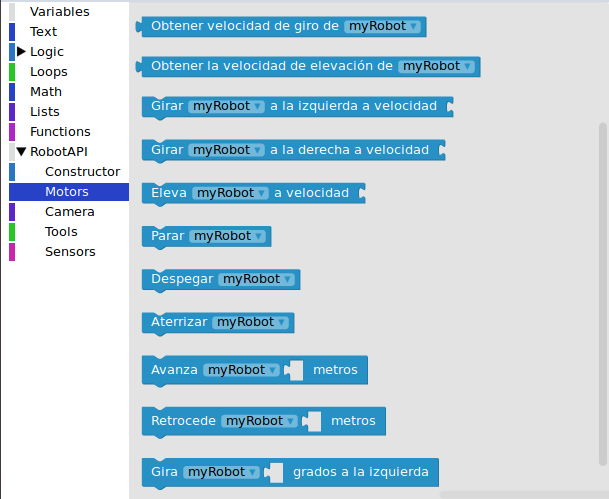
\includegraphics[width=0.65\textwidth]{img/kibotics_newblocks.png}
            \caption{Espacio de trabajo de \textit{Scratch} con los bloques del drone incorporados} 
            \label{fig:newblocks}
        \end{figure}

\subsection{Modelo 3D}

Para simular el robot en el entorno de \textit{A-Frame} es necesario realizar un modelo tridimensional. Para ello se ha buscado un modelo en una librería\footnote{\url{https://sketchfab.com/}} y se ha editado en \textit{Blender} (figura \ref{fig:droneBlender}) para que se ajuste a los requisitos del entorno. Las modificaciones que se han realizado al modelo son: 
\begin{itemize}
    \item Reducción de polinomios  para que no se ralentice la carga del mundo.
    \item Rotación del modelo para que encaje con la orientación que disponía el anterior robot. Es decir, que el robot tenga su parte frontal mirando hacia el eje X positivo para que al comandarle velocidad lineal se desplace hacia delante.
    \item Modificación de la luz para adaptarla al escenario de \textit{WebSim}. 
    
    \item Elaborar una animación a las hélices para darle un aspecto más realista. Esta animación se activa vía \textit{software} cuando el drone despega del suelo\footnote{\url{https://www.youtube.com/watch?v=XjQNhNCkOJA}}.
\end{itemize}

 \begin{figure}
    \centering
    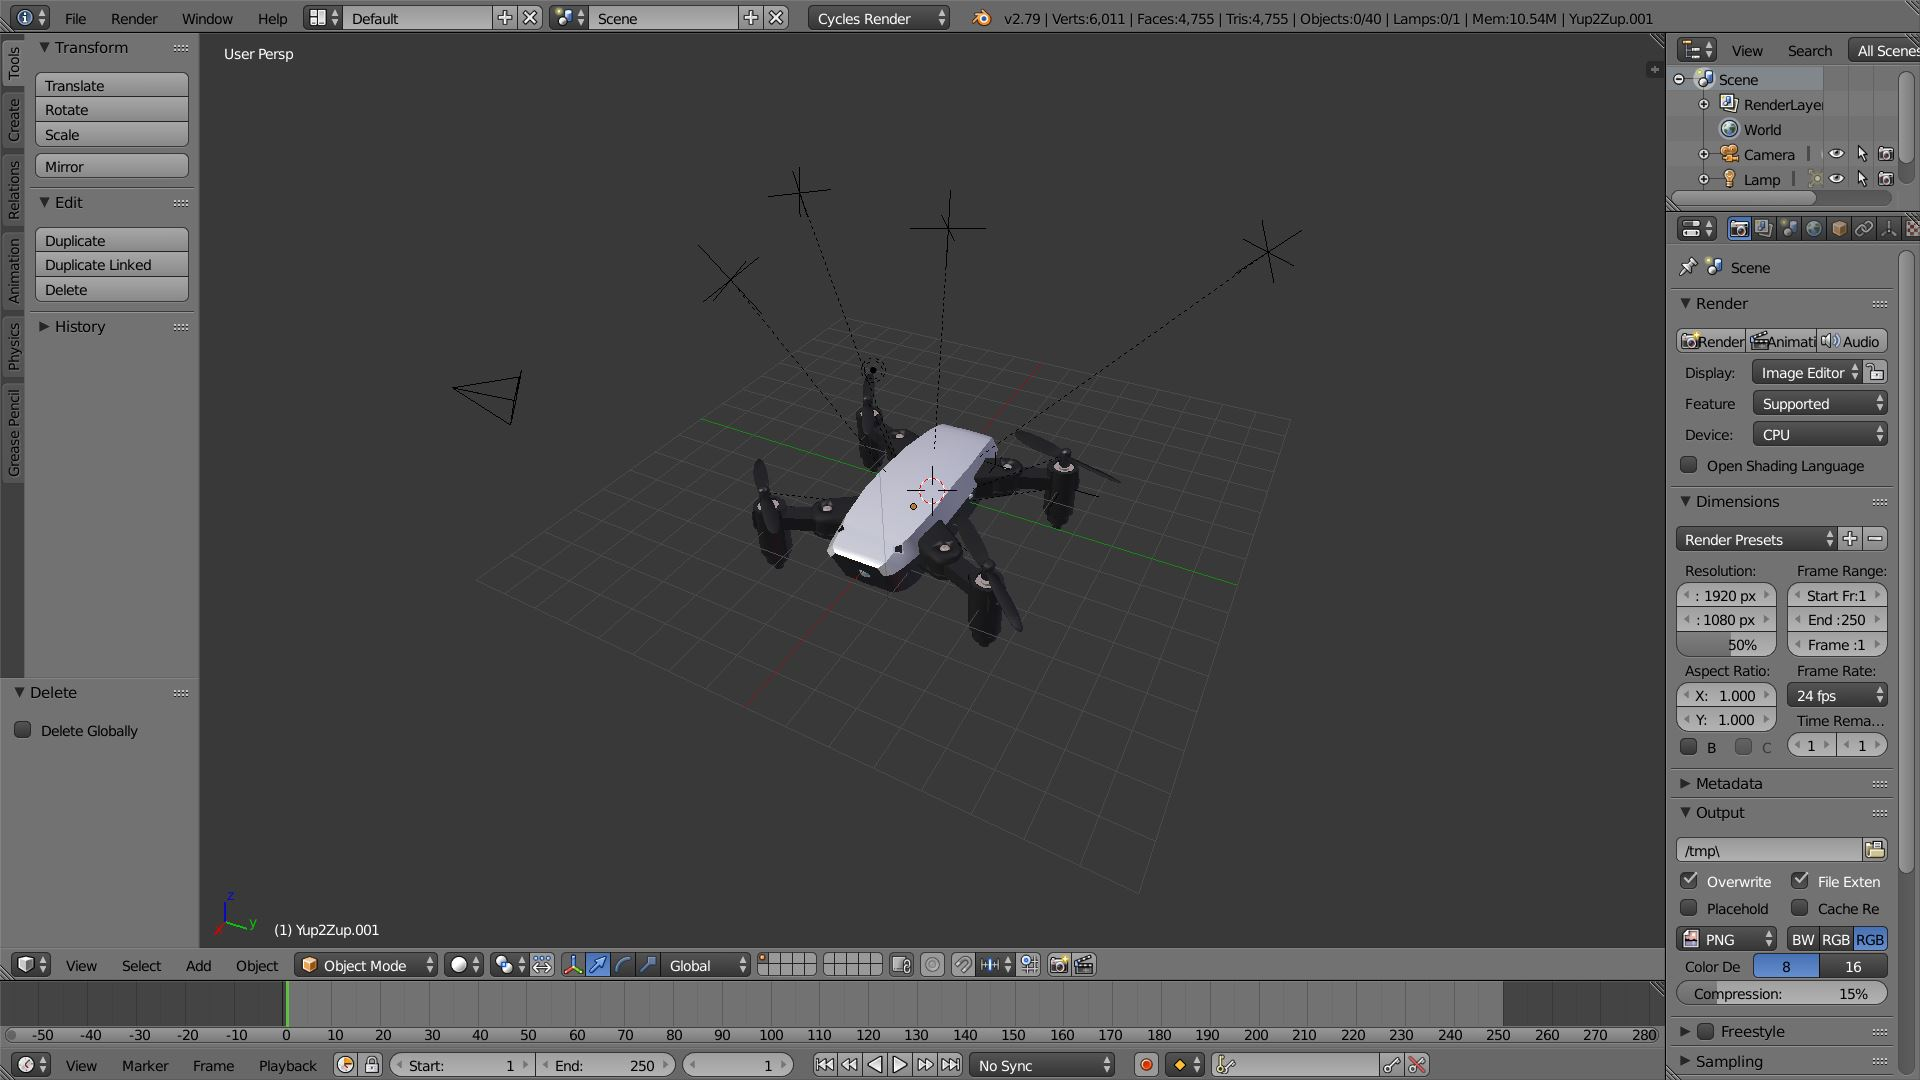
\includegraphics[scale=0.3]{img/droneBlender.jpg}
    \caption{Drone en Blender} \label{fig:droneBlender}
\end{figure}

El drone implementado en el entorno de \textit{Websim} se puede ver en la figura \ref{fig:escenarioDrone}.
   \begin{figure}[H]
    \centering
    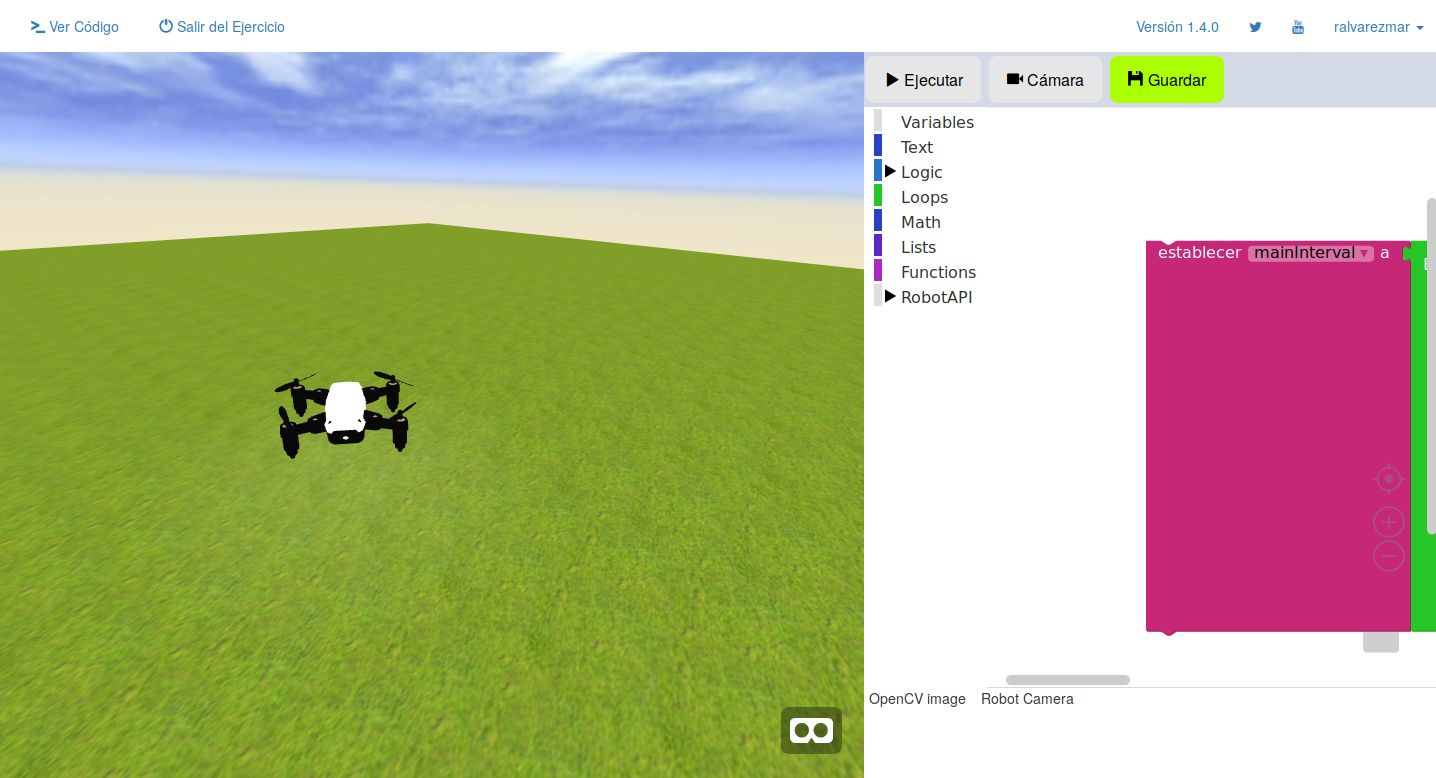
\includegraphics[scale=0.3]{img/websimDrone.png}
    \caption{Escenario de WebSim con drone integrado} \label{fig:escenarioDrone}
    \end{figure}


\section{Escenarios}

Se han incorporado nuevos escenarios a \textit{WebSim} que dan la posibilidad de realizar nuevos ejercicios o de mejorar el que había ya disponible. En esta sección se explicarán los escenarios con un solo robot y se hará mención a los escenarios con dos robots, que se explicarán en profundidad más adelante.

\subsection{Sigue-líneas visión}
    Se ha mejorado el escenario cambiando la textura del suelo a una creada con la trazada del circuito de Interlagos. Se ha realizado con un programa de diseño gráfico y, debido a su peso, se ha reducido posteriormente su tamaño para aliviar los tiempos de carga. 
    
    \begin{figure}[H]
    \centering
    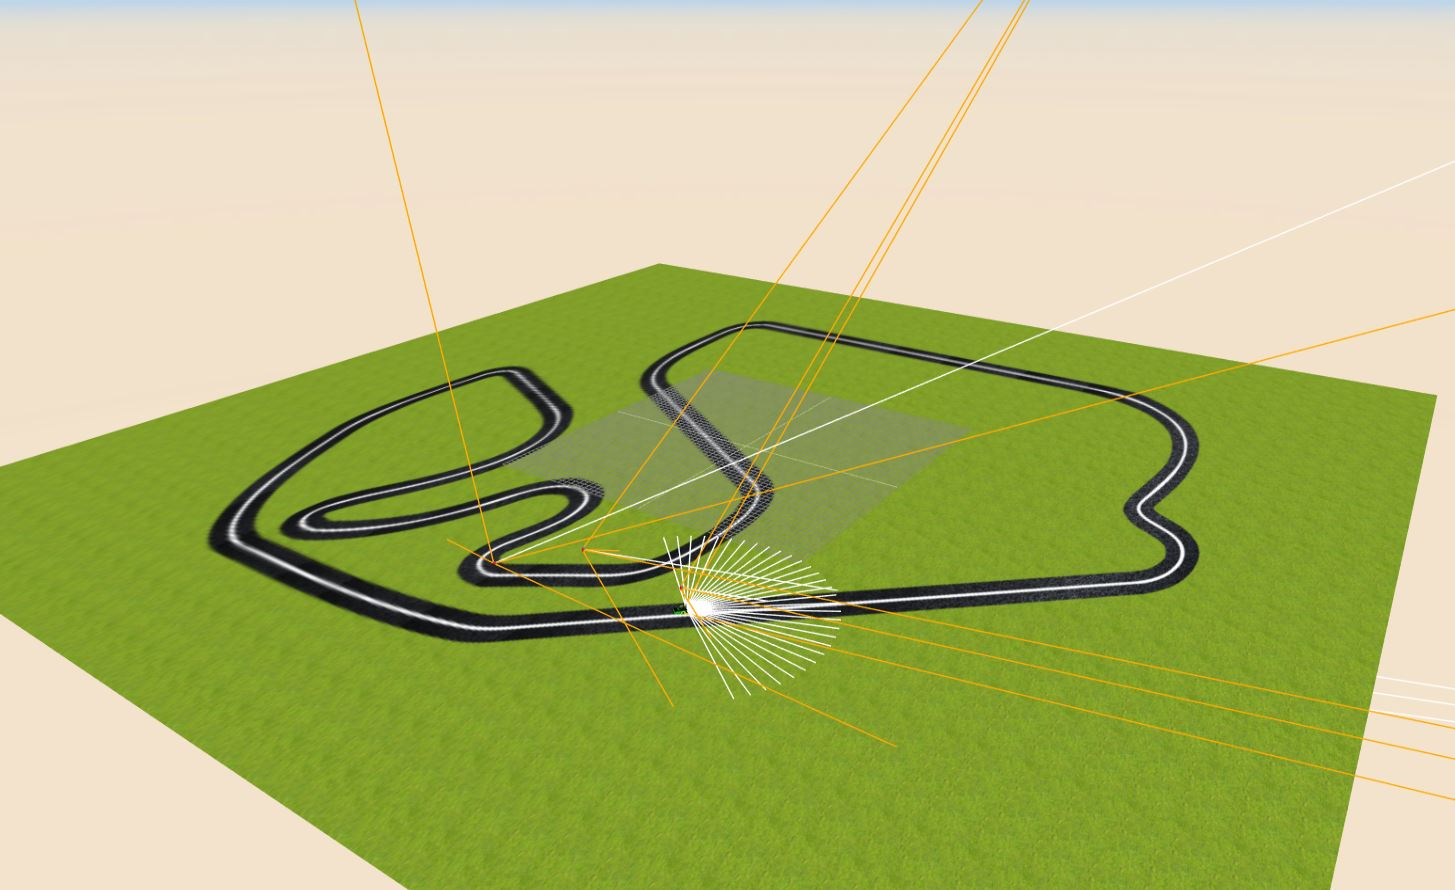
\includegraphics[scale=0.4]{img/pibot_vision.JPG}
    \caption{Escenario para el ejercicio \textit{piBot} sigue-líneas con cámara} \label{fig:siguelineavision}
    \end{figure}
    
\subsection{Sigue-líneas infrarrojos}
    Con un recorrido similar a sigue-líneas visión, pero con fondo blanco y recorrido negro para facilitar la implementación de código al robot real y que no haya que realizar modificaciones. Para que funcionara correctamente ha sido necesario añadir el color blanco a \textit{undestandedColors} para realizar el filtro y poder pasar ``\textit{white}'' como atributo a la función \textit{getObjectColor()}.
    
    \begin{figure}[H]
    \centering
    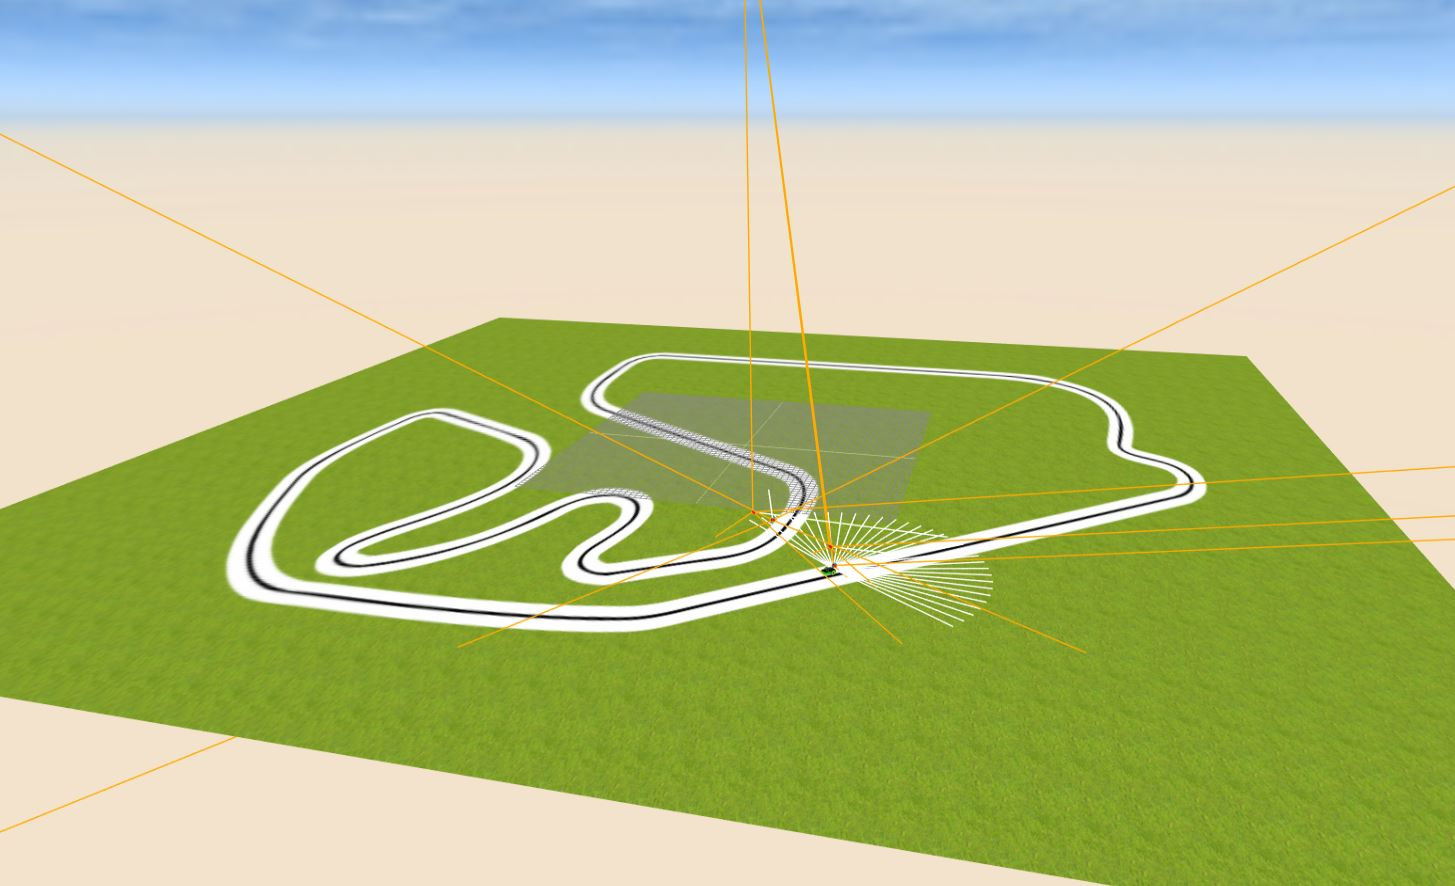
\includegraphics[scale=0.4]{img/siguelineas_ir.JPG}
    \caption{Escenario para el ejercicio \textit{piBot} sigue-líneas infrarrojo} \label{fig:siguelineasIR}
    \end{figure}
    
\subsection{Choca-gira}
Escenario creado en \textit{Blender} con un aspecto similar a su análogo en \textit{Python}. Para ello se han adaptado la mayor parte de las estructuras que dispone el escenario original para su integración en \textit{WebSim}. 

    \begin{figure}[H]
    \centering
    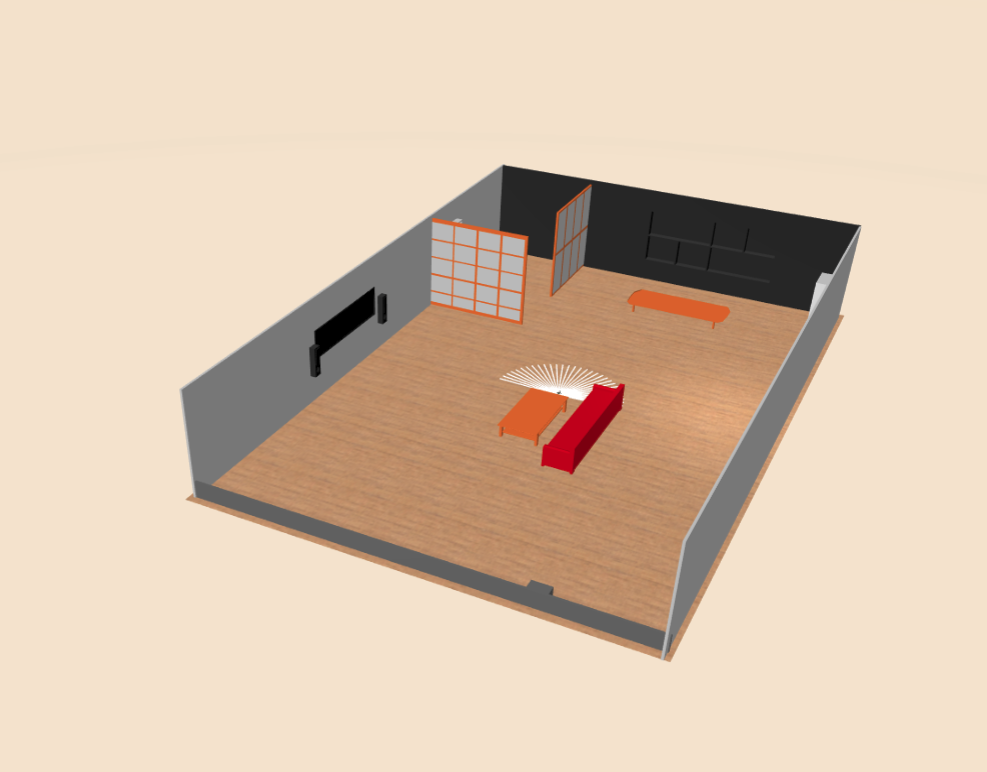
\includegraphics[scale=0.4]{img/bump&go.png}
    \caption{Escenario para el ejercicio choca-gira} \label{fig:chocagira}
    \end{figure}


\subsection{Sigue-pelota con piBot}
Dispone de una pelota de color rojo en el escenario a la que se le ha dado movimiento a través de primitivas de \textit{A-Frame}. En la figura \ref{fig:secuenciaPibot} se puede ver una secuencia con la animación de la pelota. 



\begin{figure}[htbp]
\begin{subfigure}[t]{0.2\textwidth}
    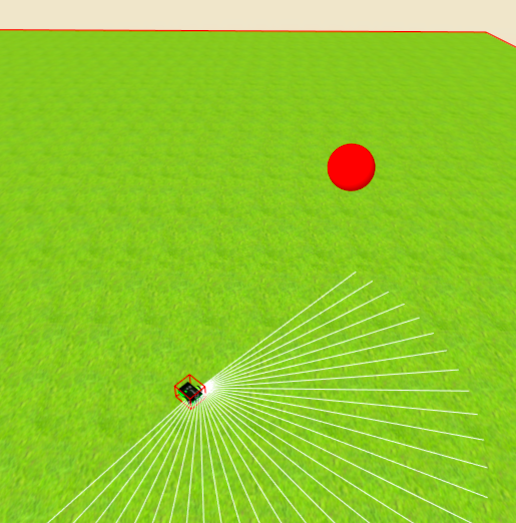
\includegraphics[width=3cm, height=3cm]{img/BallPibot1.png}
\label{fig:figure1_1}
\end{subfigure}\hfill
\begin{subfigure}[t]{0.2\textwidth}
  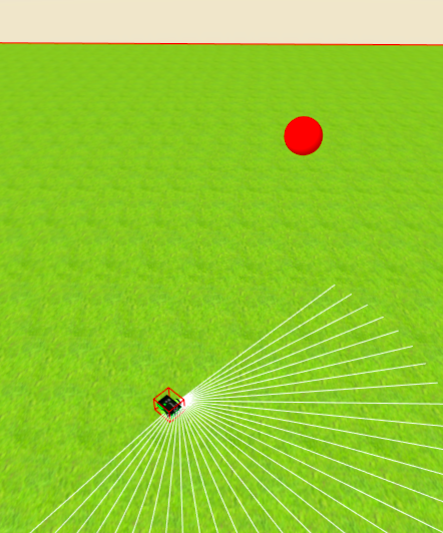
\includegraphics[width=3cm, height=3cm]{img/BallPibot2.png}
\label{fig:figure1_2}
\end{subfigure}\hfill
\begin{subfigure}[t]{0.2\textwidth}
    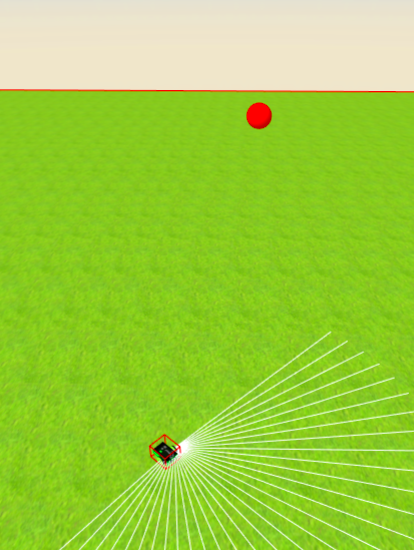
\includegraphics[width=3cm, height=3cm]{img/BallPibot3.png}
\label{fig:figure1_3}
\end{subfigure}

\begin{subfigure}[t]{0.2\textwidth}
    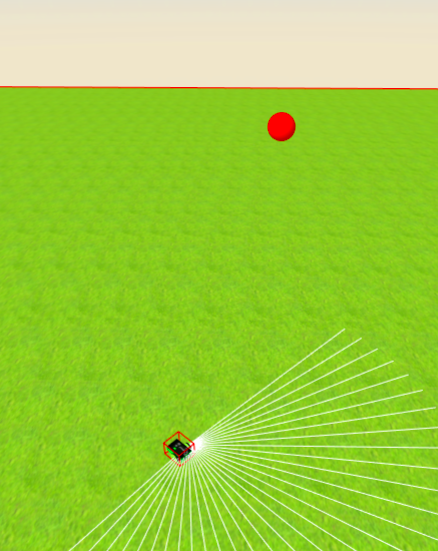
\includegraphics[width=3cm, height=3cm]{img/BallPibot4.png}
\label{fig:figure1_4}
\end{subfigure}\hfill
\begin{subfigure}[t]{0.2\textwidth}
    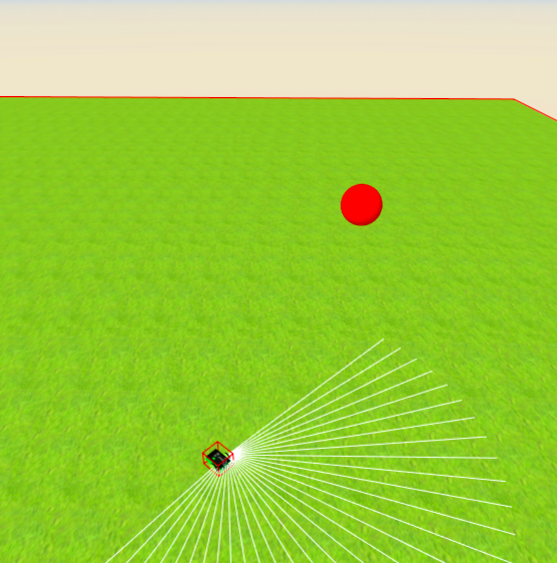
\includegraphics[width=3cm, height=3cm]{img/BallPibot5.png}
\label{fig:figure1_5}
\end{subfigure}\hfill
\begin{subfigure}[t]{0.2\textwidth}
    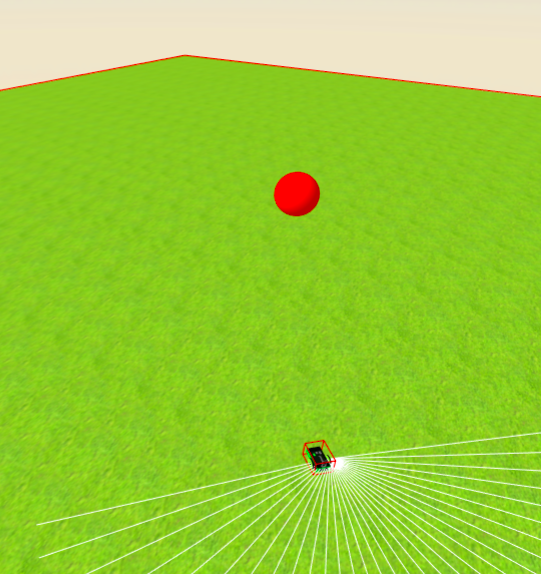
\includegraphics[width=3cm, height=3cm]{img/BallPibot6.png}
\label{fig:figure1_6}
\end{subfigure}

\begin{subfigure}[t]{0.2\textwidth}
    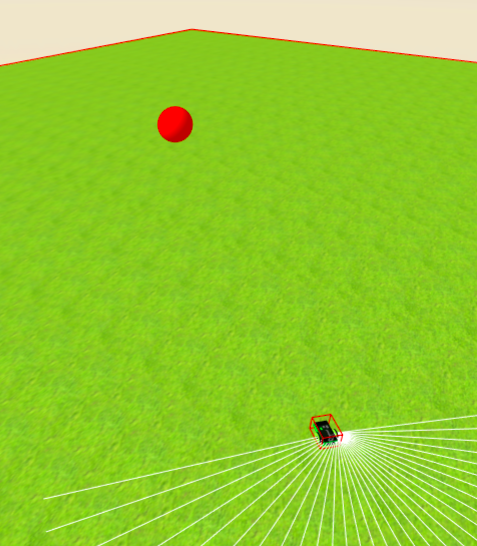
\includegraphics[width=3cm, height=3cm]{img/BallPibot7.png}
\label{fig:figure1_7}
\end{subfigure}\hfill
\begin{subfigure}[t]{0.2\textwidth}
    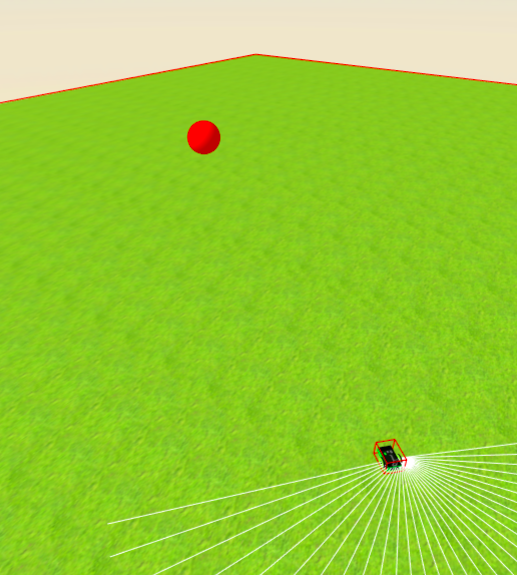
\includegraphics[width=3cm, height=3cm]{img/BallPibot8.png}
\label{fig:figure1_8}
\end{subfigure}\hfill
\begin{subfigure}[t]{0.2\textwidth}
    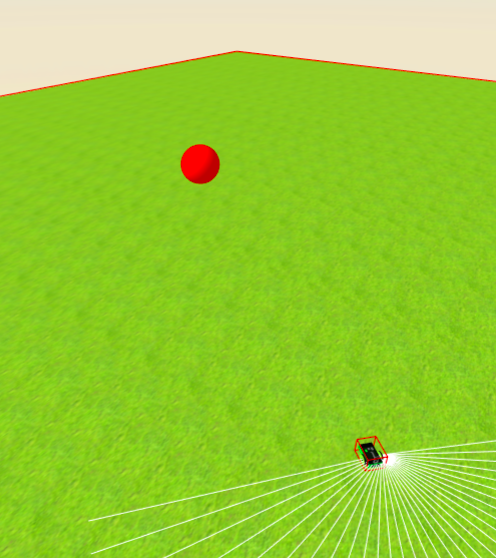
\includegraphics[width=3cm, height=3cm]{img/BallPibot9.png}
\label{fig:figure1_9}
\end{subfigure}
\caption{Secuencia de la animación de una pelota para el ejercicio piBot sigue-pelota}
\label{fig:secuenciaPibot}
\end{figure}

\subsection{Atraviesa-bosque}
Creado con primitivas de \textit{A-Frame}, el escenario tiene disposición de pasillo y diversos objetos en el camino para realizar un ejercicio que haga uso del sensor de ultrasonidos para evitar obstáculos.

    \begin{figure}[H]
    \centering
    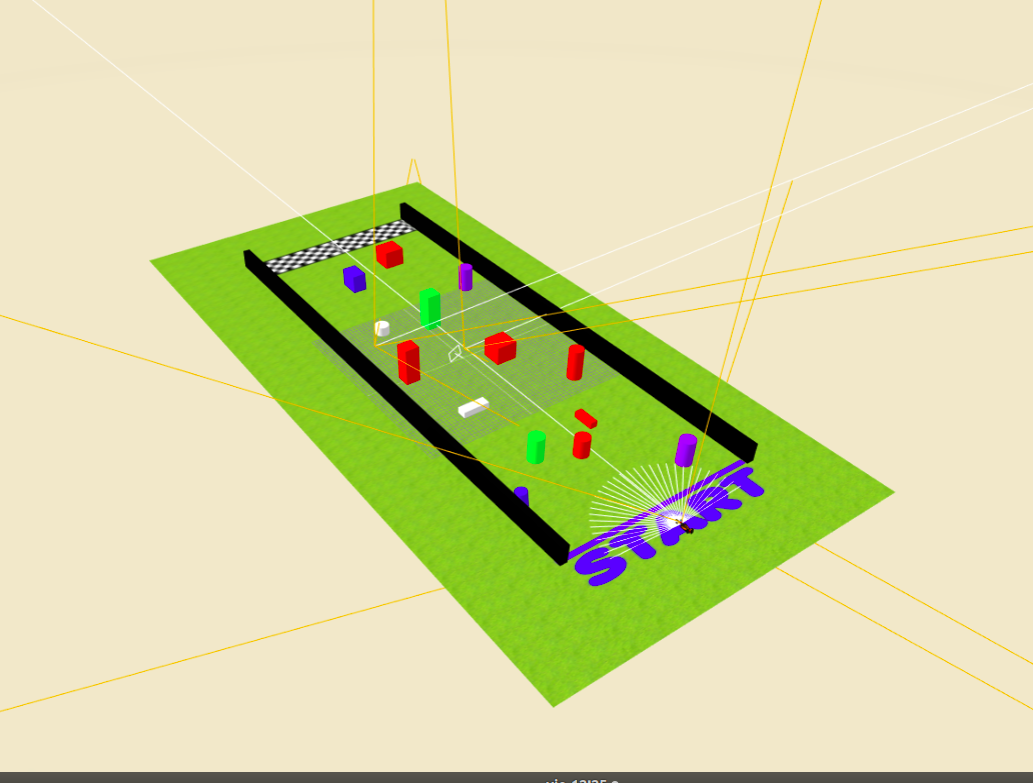
\includegraphics[scale=0.4]{img/atraviesabosque-indiv.png}
    \caption{Escenario para el ejercicio atraviesa bosque} 
    \label{fig:atraviesaBosqueind}
    \end{figure}
    
\subsection{Sigue-pelota con drone}
Realizado de forma similar al ejercicio con piBot, pero modificando la animación para que la pelota se mueva también en el eje Y. Se puede ver una secuencia con la animación en la figura \ref{fig:secuenciaDrone}.


\begin{figure}[htbp]
\begin{subfigure}[t]{0.2\textwidth}
    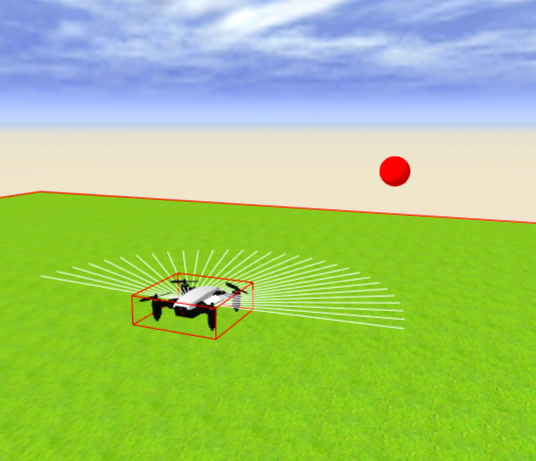
\includegraphics[width=3cm, height=3cm]{img/followBallTello1.png}
\label{fig:figure2_1}
\end{subfigure}\hfill
\begin{subfigure}[t]{0.2\textwidth}
  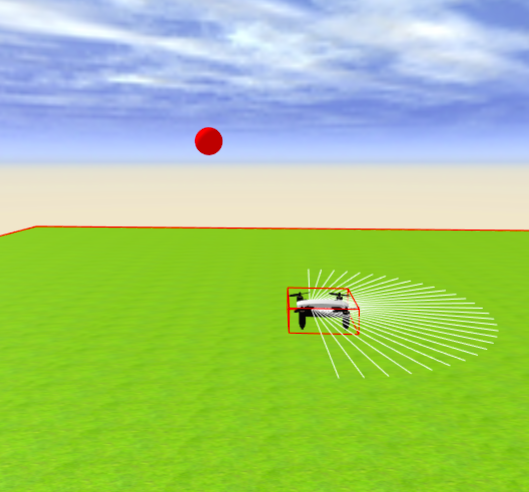
\includegraphics[width=3cm, height=3cm]{img/followBallTello2.png}
\label{fig:figure2_2}
\end{subfigure}\hfill
\begin{subfigure}[t]{0.2\textwidth}
    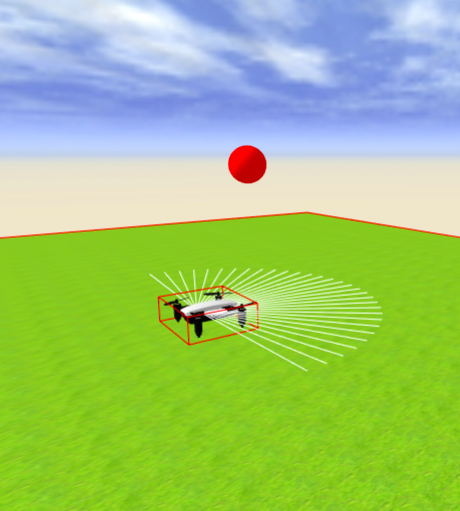
\includegraphics[width=3cm, height=3cm]{img/followBallTello3.png}
\label{fig:figure2_3}
\end{subfigure}

\begin{subfigure}[t]{0.2\textwidth}
    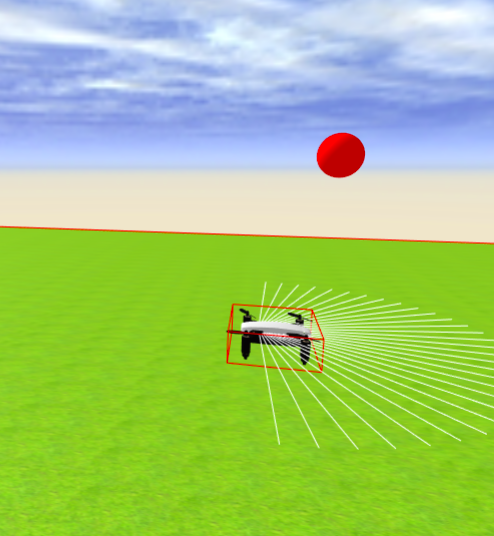
\includegraphics[width=3cm, height=3cm]{img/followBallTello4.png}
\label{fig:figure2_4}
\end{subfigure}\hfill
\begin{subfigure}[t]{0.2\textwidth}
    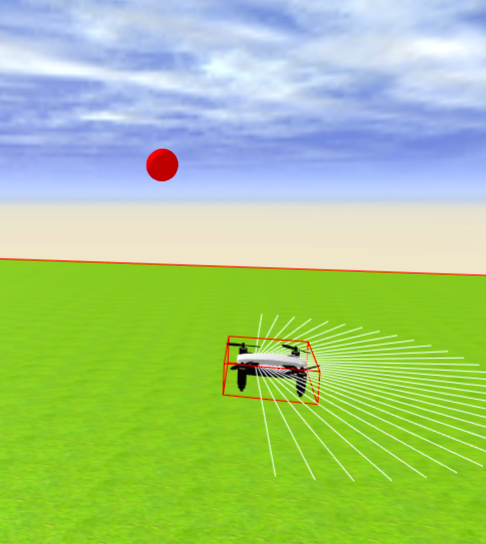
\includegraphics[width=3cm, height=3cm]{img/followBallTello5.png}
\label{fig:figure2_5}
\end{subfigure}\hfill
\begin{subfigure}[t]{0.2\textwidth}
    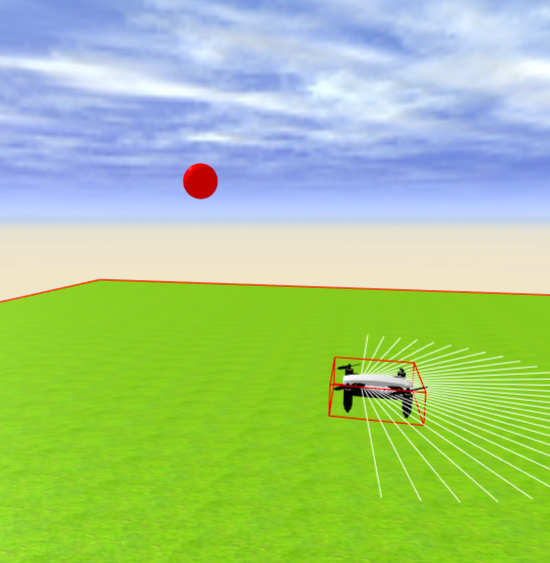
\includegraphics[width=3cm, height=3cm]{img/followBallTello6.png}
\label{fig:figure2_6}
\end{subfigure}

\begin{subfigure}[t]{0.2\textwidth}
    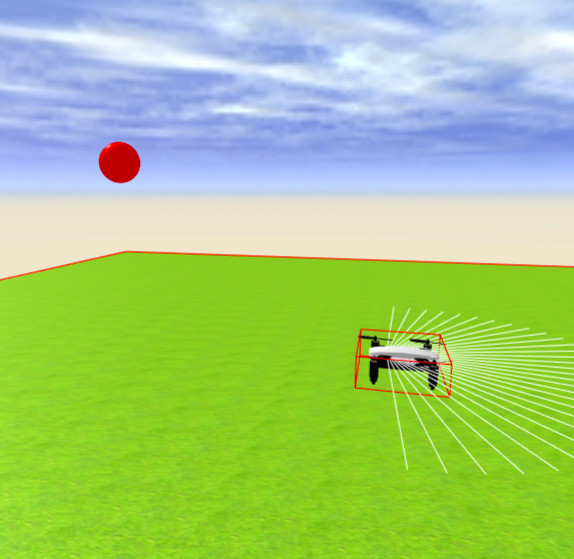
\includegraphics[width=3cm, height=3cm]{img/followBallTello7.png}
\label{fig:figure2_7}
\end{subfigure}\hfill
\begin{subfigure}[t]{0.2\textwidth}
    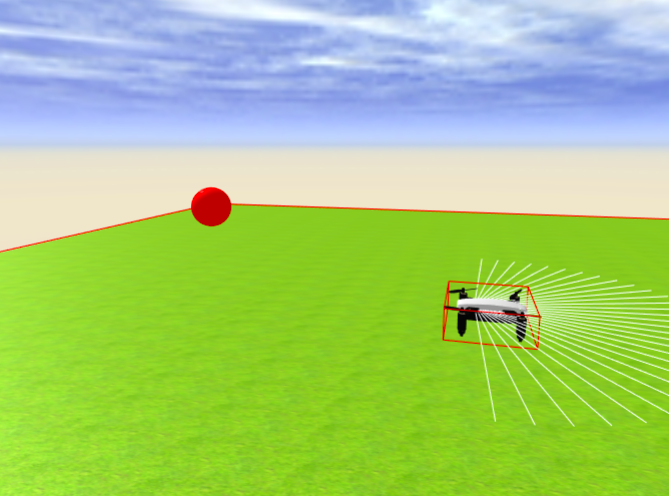
\includegraphics[width=3cm, height=3cm]{img/followBallTello8.png}
\label{fig:figure2_8}
\end{subfigure}\hfill
\begin{subfigure}[t]{0.2\textwidth}
    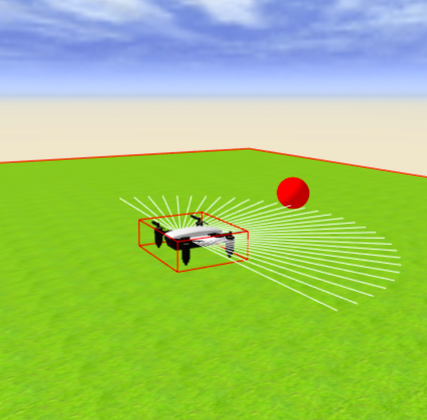
\includegraphics[width=3cm, height=3cm]{img/followBallTello9.png}
\label{fig:figure2_9}
\end{subfigure}

\begin{subfigure}[t]{0.2\textwidth}
    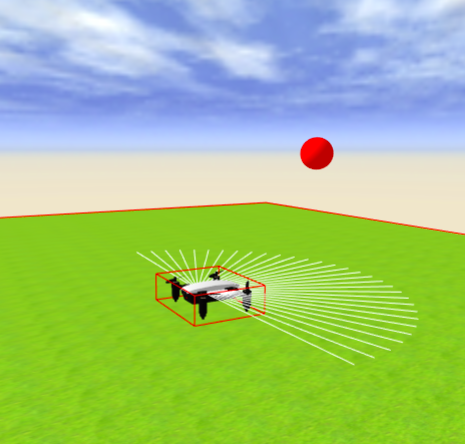
\includegraphics[width=3cm, height=3cm]{img/followBallTello10.png}
\label{fig:figure2_10}
\end{subfigure}\hfill
\begin{subfigure}[t]{0.2\textwidth}
    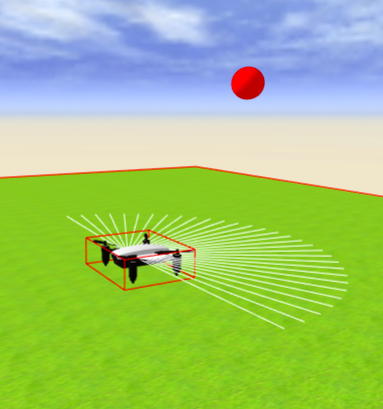
\includegraphics[width=3cm, height=3cm]{img/followBallTello11.png}
\label{fig:figure2_11}
\end{subfigure}\hfill
\begin{subfigure}[t]{0.2\textwidth}
    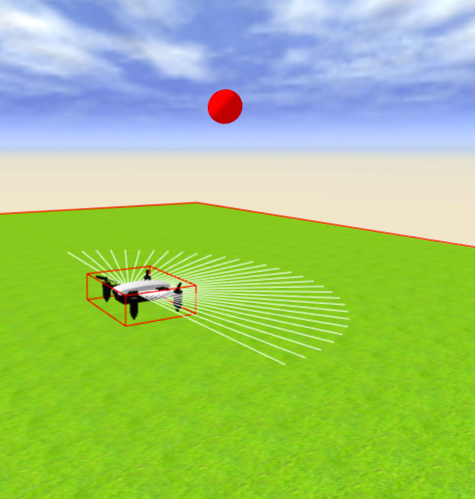
\includegraphics[width=3cm, height=3cm]{img/followBallTello12.png}
\label{fig:figure2_12}
\end{subfigure}
\caption{Secuencia de la animación de una pelota para el ejercicio \textit{drone} sigue-pelota}
\label{fig:secuenciaDrone}
\end{figure}

\subsection{Cuadrado con drone}

Escenario para facilitar el ejercicio ``cuadrado drone'' en el que hay que dibujar un cuadrado con el movimiento del \textit{drone}.
    
    \begin{figure}[H]
        \centering
        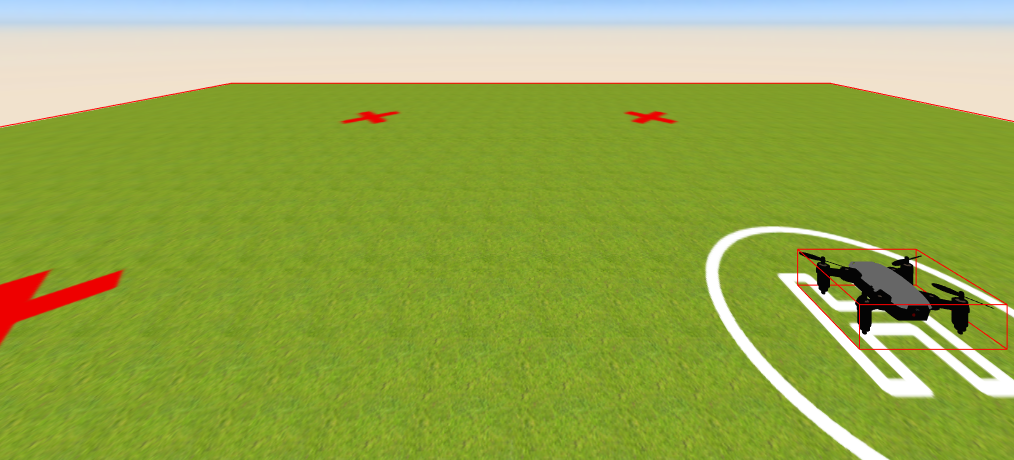
\includegraphics[scale=0.4]{img/cuadradoDrone.png}
        \caption{Escenario de WebSim para el ejercicio drone cuadrado} 
        \label{fig:droneCuadrado}
    \end{figure}
    
\subsection{Escenarios competitivos}

Se han realizado varios escenarios para realizar ejercicios competitivos:
\begin{itemize}
    \item Muros: prototipo creado para realizar pruebas comandando velocidades a los robots y comprobar el estado de sus sensores.
      
       \begin{figure}[H]
        \centering           
        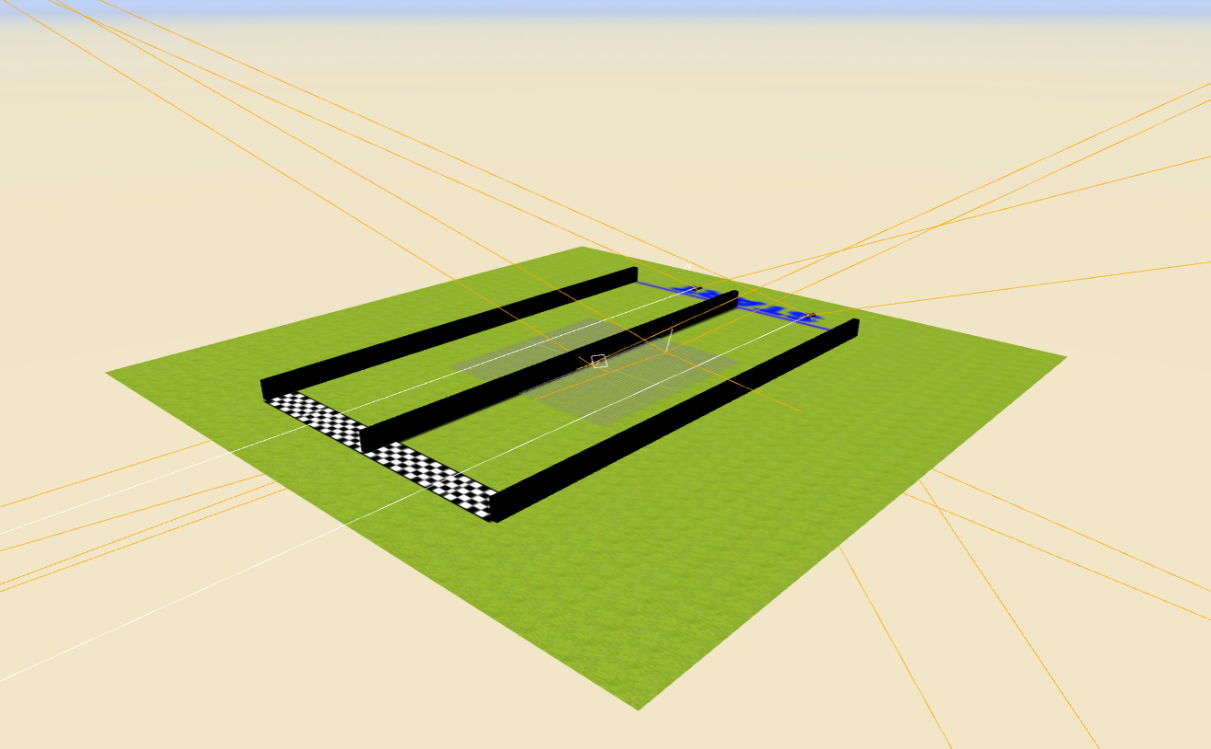
\includegraphics[scale=0.3]{img/ejercicio_muros.png}
        \caption{Prototipo ejercicio competitivo}
        \label{fig:ejercicio_muro}
    \end{figure}

    
    \item Atraviesa-bosque: ejercicio similar al escenario con un solo robot, pero en este caso se han creado dos pasillos con objetos para recorrerlos sin chocar con ninguno de los obstáculos. Se han añadido distintas primitivas de \textit{A-Frame} en la misma ubicación para los dos \textit{robots} para que el recorrido sea justo.
    
    \begin{figure}[H]
        \centering           
        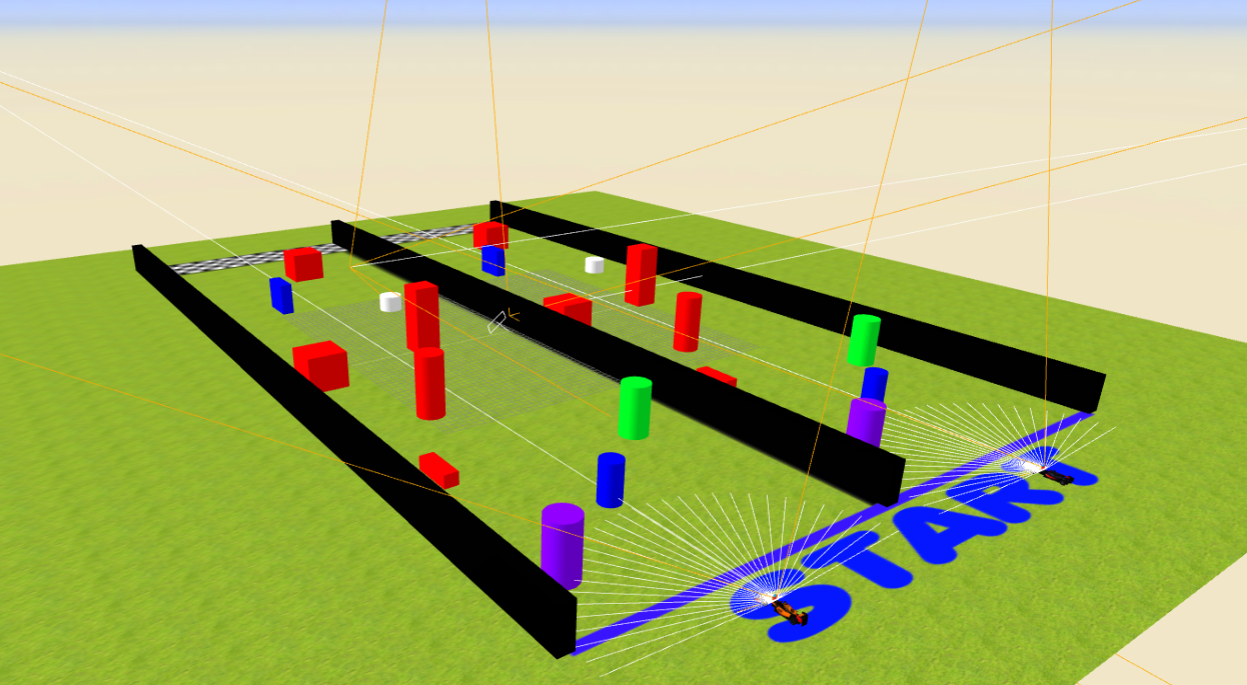
\includegraphics[scale=0.3]{img/ejercicio_atraviesabosque.png}
        \caption{Ejercicio atraviesa-bosque competitivo}
        \label{fig:atraviesabosque_escenario}
    \end{figure}
    
    \item Sigue-líneas: escenario con dos robots en el que tienen que seguir una linea de color blanco sobre fondo negro atravesando un puente en medio del circuito para que, de esta manera, ambos recorran la misma distancia.

    \begin{figure}[H]
        \centering            
        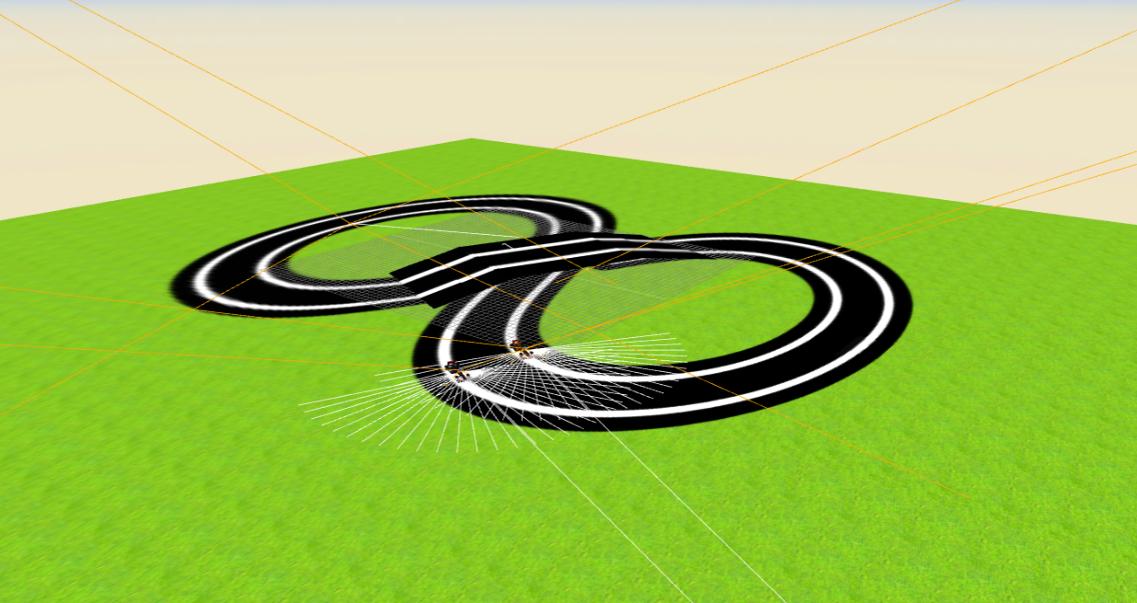
\includegraphics[scale=0.3]{img/ejercicio_siguelineas.png}
        \caption{Ejercicio sigue-líneas competitivo}
        \label{fig:siguelineas_competitivo}
    \end{figure}
\end{itemize}

Siendo el principal problema el puente creado para el ejercicio sigue-líneas. La solución definitiva ha sido creando primitivas de \textit{A-Frame} (\textit{a-plane}) de tal forma que simule un puente y pueda cruzarlo el coche. Se ha intentado realizar un modelo de puente en \textit{Blender}, pero el entorno no simulaba correctamente la malla de colisiones siendo imposible subir el puente porque el robot ``chocaba'' contra él. En la figura \ref{fig:prueba_puente} se puede ver el puente creado y la malla de colisión generada por \textit{A-Frame}.

    \begin{figure}[H]
        \centering            
        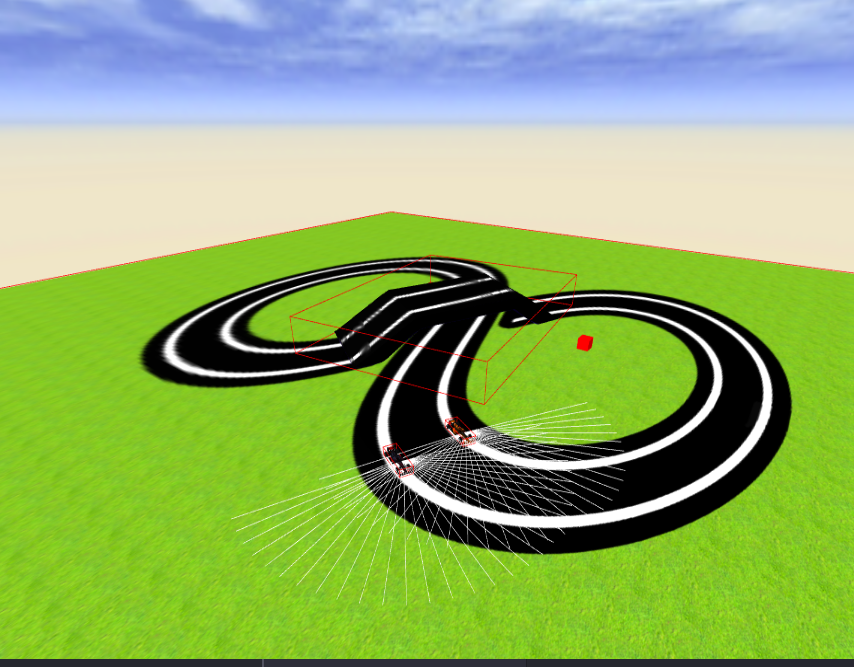
\includegraphics[scale=0.3]{img/prueba_puente.png}
        \caption{Prueba de puente creado en \textit{Blender}}
        \label{fig:prueba_puente}
    \end{figure}


\section{Teleoperadores}
Se han incorporado teleoperadores en \textit{WebSim} para poder controlar los robots sin necesidad de programarlos. De esta manera es posible saber el estado y valor de sus sensores de manera sencilla ayudando a los desarrolladores a buscar fallos en drivers o incorporar nuevos escenarios. 

\subsection{Ficheros de configuración}

Para incorporar estos teleoperadores ha sido necesario elaborar unos ficheros de configuración y así poder cambiar el escenario y el \textit{drone} cargado por \textit{A-Frame}. 

Estos archivos de configuración se han creado en \textit{JSON} (un formato de texto para representar datos estructurados en la sintaxis de objeto de \textit{JavaScript}) y se ha programado un \textit{script} para cargar cada fichero de configuración. Para ello se crea una variable en el \textit{index.html} del editor con la ruta en la que esté ubicado y el \textit{script} abre el fichero y recorre el \textit{JSON} para dar al escenario los valores establecidos. \newline

En los ficheros creados se pueden configurar aspectos como el modelo del robot cargado, su posición y rotación, la posición de la cámara a bordo del robot, el fichero del cielo y suelo que debe cargar o los elementos que queramos añadir en el escenario. \newline

\begin{lstlisting}[language=json, caption=Ejemplo de fichero de configuración]
  {
  "robot": {
    "model":"../assets/models/drone.gltf",
    "scale": "0.5 0.5 0.5",
    "position":"12 0 25",
    "rotation": "0 320 0"
  },
  "gravity": 0,
  "ground": "../assets/textures/escenarioLiso.png",
  "sky": "../assets/textures/sky.png",
  "secondaryCamera": "0 0 0",
  "cameraRobot":"0 0.03 -0.01",
  "objects":[{
      "type": "a-sphere",
      "position": "4 1 20",
      "color": "#FF0000"
      }
    ]
}
\end{lstlisting}

En este ejemplo se configura el escenario para que cargue el modelo del \textit{drone}, con el tamaño indicado en \textit{size}, la posición y rotación que aparece en \textit{position} y \textit{rotation}. En el valor \textit{gravity} se indica que el escenario no tenga gravedad, se carga la textura que posee el campo \textit{ground} como suelo del mundo y, por último, la posición de las cámaras es la ubicada en \textit{secondaryCamera} y \textit{cameraRobot}. Además, en \textit{objects} se pueden añadir todos los objetos deseados a la escena. En este ejemplo se añade una pelota de color rojo en la posición que aparece en \textit{position}.

\subsection{Teleoperadores}

Además de los modelos existentes del drone y \textit{piBot}, se han creado otros nuevos para extender las posibilidades de la plataforma y poder teleoperar todos ellos.
\begin{figure}[H]
    \centering            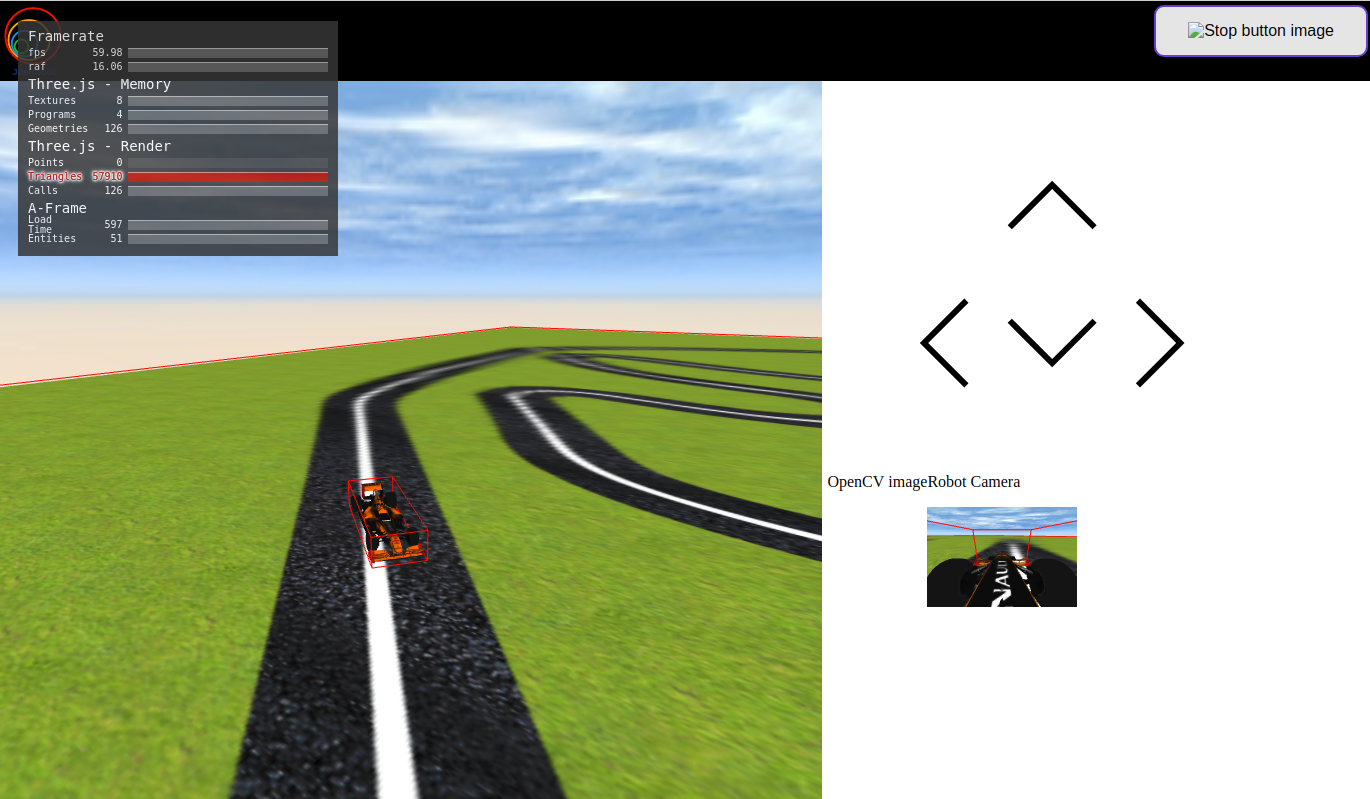
\includegraphics[scale=0.35]{img/f1_teleoperator.png}
    \caption{Teleoperador para el modelo del fórmula 1} \label{fig:f1_teleoperator}
\end{figure}
\begin{figure}[H]
    \centering            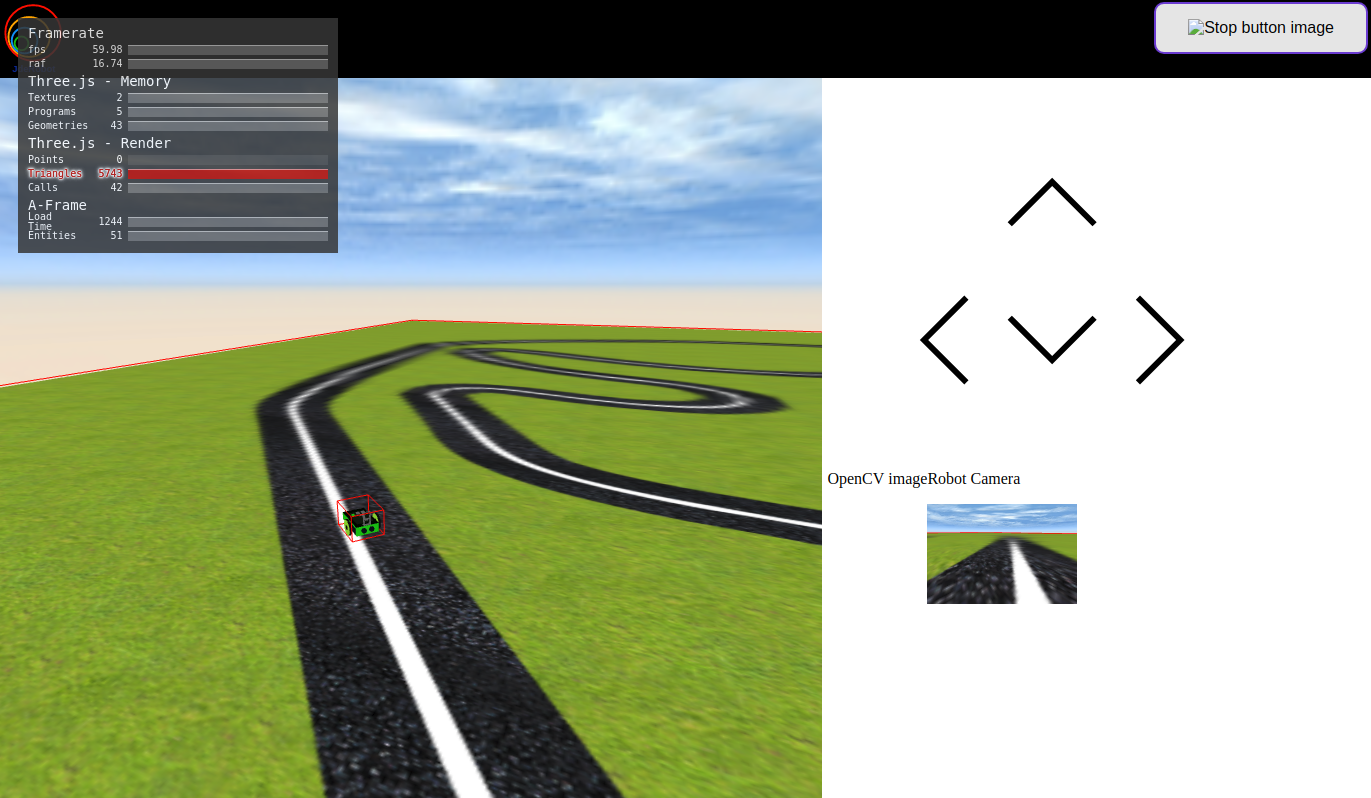
\includegraphics[scale=0.35]{img/pibot_teleoperator.png}
    \caption{Teleoperador para el modelo del piBot} \label{fig:piBot_teleoperator}
\end{figure}
  \begin{figure}[H]
    \centering
    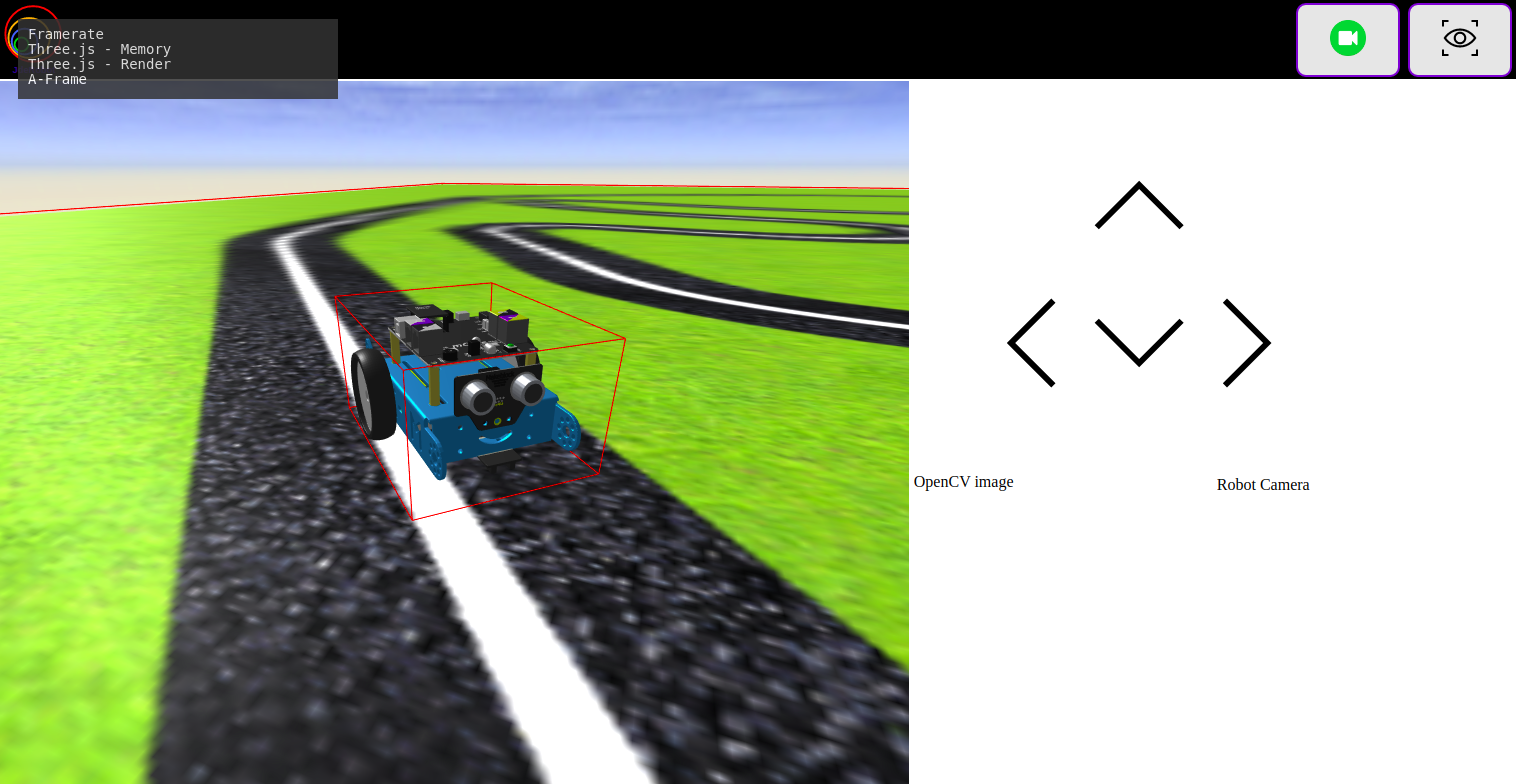
\includegraphics[scale=0.3]{img/mBot_teleoperator.png}
    \caption{Teleoperador para el modelo del mBot} \label{fig:mBot_teleoperator}
\end{figure}
\begin{figure}[H]
    \centering
    \includegraphics[scale=0.3]{img/drone_teleoperator.png}
    \caption{Teleoperador para el modelo del drone} \label{fig:drone_teleoperator}
\end{figure}
    
Pudiendo controlar todos ellos con los botones que aparecen en la imagen o bien a través del teclado. 
Además, se ha creado una página principal para poder acceder a todos ellos a través de una interfaz gráfica: 

 \begin{figure}[H]
    \centering
    \includegraphics[scale=0.25]{img/teleoperators.png}
    \caption{Interfaz que permite acceder a cada uno de los teleoperadores} \label{fig:teleoperators}
\end{figure}

\section{Ejercicios competitivos}

Uno de los objetivos de este proyecto era añadir ejercicios competitivos. Se hace especial mención a ellos debido a que son completamente diferentes al resto de los ya creados. Este tipo de ejercicios aumenta el valor de la plataforma ya que da la posibilidad de programar dos robots en el mismo escenario, pudiendo entender la programación como un juego en el que se premia al que aporte la mejor solución.

%  Para dar soporte a este tipo de ejercicios se ha realizado una refactorización de \textit{WebSim}, actualizando así la aplicación a la versión \textit{WebSim 2.0}. En esta versión se separan los hilos de \textit{HAL API}, simulador y editor dando la posibilidad de crear más de un robot en la misma escena, cambiar el código del robot en la simulación o incluso parar la simulación y reanudarla después con un código distinto. \newline

En este tipo de ejercicios hay dos robots en una misma escena donde cada uno de ellos se puede programar con un código distinto. Para facilitar la integración con el resto de la plataforma se han incorporado dos aplicaciones más a \textit{WebSim}: ejercicios competitivos en \textit{Scratch} y ejercicios competitivos en \textit{JavaScript}. 


Se ha comenzado creando la aplicación llamada \textit{competitive-JavaScript} debido a la facilidad para probar código y hacer pruebas en el entorno. Para ello se ha cambiado la interfaz del editor, añadiendo botones para cada uno de los robots (figura \ref{fig:javascript_competitivo}) y añadir funcionalidad a cada botón para guardar el código de cada robot o mostrar el código en caso de tener uno guardado.

    \begin{figure}[h]
        \centering            \includegraphics[scale=0.30]{img/competitiveEditorJavascript.png}
        \caption{Editor de \textit{JavaScript} para ejercicios competitivos}
        \label{fig:javascript_competitivo}
    \end{figure}

La aplicación \textit{competitive-Scratch} se ha realizado de la misma manera, con la diferencia de que, en este caso, es necesario guardar el código de los bloques en \textit{XML} y su traducción en \textit{JavaScript}. Para realizarlo de forma limpia se ha creado un objeto que contiene un \textit{boolean} y dos cadenas de texto. En el \textit{boolean} se indica el código de qué \textit{robot} se está editando, en una cadena de texto se guarda el código \textit{XML} y en la otra su traducción en \textit{JavaScript}. Se puede ver la interfaz de este editor en la figura \ref{fig:scratch_competitivo}.

    \begin{figure}[h]
        \centering            
        \includegraphics[scale=0.30]{img/competitivoEditorScratch.png}
        \caption{Editor de \textit{Scratch} para ejercicios competitivos}
        \label{fig:scratch_competitivo}
    \end{figure}
    
Para puntuar el comportamiento de los robots de manera justa, se han incluido en estos ejercicios evaluadores automáticos. Van a tener diferentes comportamientos en cada ejercicio, por lo que se han desarrollado de tal forma que se pueda cargar cargar un evaluador distinto para cada uno o, incluso, no cargar ninguno. \newline

Para su implementación se ha creado la función \textit{runEvaluator}, que acepta como parámetro un \textit{array} con los identificadores de los robots y el archivo del evaluador deseado. Este fichero se recoge como variable en el \textit{index.html} del editor correspondiente (de forma similar a los archivos de configuración). 
Para llamar a \textit{runEvaluator} se comprueba que se haya pasado un fichero en el \textit{index.html} y, si eso ocurre, se realiza un \textit{require} de ese fichero y se ejecuta la función principal del evaluador, \textit{evaluator.main()}, que se encarga de llamar a las funciones necesarias para que el evaluador sea completo: crea la interfaz gráfica y la funcionalidad necesaria para su correcto funcionamiento. 

A continuación se explican los ejercicios y evaluadores para cada uno de ellos. 

\subsection{Atraviesa-bosque competitivo}

Para este ejercicio se usa el escenario de la imagen \ref{fig:atraviesabosque_escenario}. Se ha creado un evaluador en el que se crea una barra de progreso para cada robot y un cronómetro. Cuando se empiezan a mover los robots la barra de progreso se va completando y el cronómetro se inicia, para comprobar el porcentaje completado solo hay que obtener la posición del robot y compararla con el punto de llegada.

\begin{figure}[H]
\centering           
\includegraphics[scale=0.3]{img/evaluador_forest.png}
\caption{Evaluador para el ejercicio atraviesa-bosque}
\label{fig:evaluador_bosque}
\end{figure}


\subsection{Sigue-líneas competitivo}

Para este ejercicio se usa el escenario de la figura \ref{fig:siguelineas_competitivo} y su evaluador es similar al de atraviesa-bosque con la diferencia de que es necesario guardar en todo momento la posición y distancia recorrida por cada robot para calcular el porcentaje del circuito completado.


\begin{figure}[H]
    \centering           
    \includegraphics[scale=0.3]{img/evaluator_follow_line.png}
    \caption{Evaluador sigue-líneas}
    \label{fig:evaluador_siguelineas}
\end{figure}

\subsection{Gato-ratón}

Con la nueva estructura de \textit{WebSim} se permite realizar el ejercicio gato-ratón con \textit{drones}. Se trata de otro tipo en el que no se compite con dos códigos programados por distintos usuarios, si no que un \textit{drone} ya está programado y el usuario solo tiene que desarrollar su solución para que el \textit{robot} no se aleje del objetivo. Para ello ha sido necesario crear un modelo al que se le ha pintado de color rojo para que sea más sencillo su filtrado. Se puede ver el escenario con ambos \textit{drones} en la figura \ref{fig:gato_raton}.




Para el evaluador de este ejercicio se crea un gráfico con ayuda de una librería externa de \textit{JavaScript} (\textit{JavaScript Graphics Library}\footnote{\url{http://www.jsgl.org/}}) que muestra la distancia entre \textit{drones} y el tiempo que lleva de ejecución. Se puede ver este evaluador en la figura \ref{fig:evaluador_gato_raton}.
  
    \begin{figure}[h]
    \centering           
    \includegraphics[scale=0.3]{img/ejercicio_gatoraton.png}
    \caption{Ejercicio gato-ratón}
    \label{fig:gato_raton}
    
\end{figure}
\begin{figure}[h]
\centering           
\includegraphics[scale=0.3]{img/evaluador_drone.png}
\caption{Evaluador para ejercicio gato-ratón}
\label{fig:evaluador_gato_raton}
\end{figure}


% CONCLUSIONES %
%%%%%%%%%%%%%%%%%%%%%%%%%%%%%%%%%%%%%%%%%%%%%%%%%%%%%%%%%%%%%%%%%%%%%%%%%%%%%%%%
\chapter{Conclusiones}
\label{chap:conclusiones}

Tras detallar las mejoras aportadas a \textit{WebSim}, en este capítulo se recopilan los objetivos alcanzados, se valoran los conocimientos adquiridos y se exponen las posibles líneas de mejora y extensión de la plataforma. 
\section{Conclusiones}

Repasando los objetivos establecidos en el capítulo \ref{chap:objetivos} se puede concluir que se han conseguido llevar a cabo todos los puntos establecidos. 

El primer objetivo consistía en añadir soporte a \textit{drone}  en \textit{WebSim}. En la sección \ref{sec:drone} se explica como se ha llevado a cabo este objetivo aportando el modelo en 3D, drivers y bloques para las nuevas funciones. \\

El segundo objetivo era incluir más ejercicios a \textit{WebSim}. Los nuevos escenarios se han explicado en la sección \ref{sec:escenarios} y otorga a la plataforma el poder realizar nuevos ejercicios como choca-gira (subsección \ref{subsec:chocagira}), sigue-pelota (subsecciones \ref{subsec:pelotapibot} y \ref{subsec:pelotadrone}) y atraviesa-bosque (subsección \ref{subsec:atraviesabosque}).  \\

El tercer objetivo consistía en añadir teleoperadores, que se explica en la sección \ref{sec:teleoperadores} y, además, se han creado archivos de configuración para poder cambiar de escenario y facilitar así su integración en servidor. En esta sección también se muestran los nuevos modelos creados (Fórmula 1 y mBot). \\

El último objetivo, ejercicios competitivos, se ha llevado a cabo en la sección \ref{sec:competitive}. Se han incorporado dos robots a este tipo de ejercicios (a excepción del ejercicio gato-ratón) incluyendo un nuevo modelo de Fórmula 1 y de \textit{drone} y además, se ha incorporado un evaluador automático por cada ejercicio. Estos evaluadores se han realizado  \\

Además, en el desarrollo de este proyecto, se ha llevado a cabo una refactorización de \textit{WebSim} actualizando así la aplicación a la versión \textit{WebSim 2.0}. En esta versión se separan los hilos de \textit{HAL API}, simulador y editor dando la posibilidad de crear más de un robot en la misma escena, cambiar el código del robot en la simulación o, incluso, parar la simulación y reanudarla después con un código distinto. Se ha formado parte de ella con elementos como \textit{brains}, que ejecuta la inteligencia de los \textit{robots} que haya en el mundo; refactorizando los editores disponibles (editor \textit{JavaScript}, editor \textit{Scratch}, editor competitivo \textit{JavaScript}, editor competitivo \textit{Scratch} y teleoperadores) para su correcto funcionamiento o realizando pruebas y ajustes para optimizar el rendimiento de la aplicación.

\section{Mejoras futuras}


Como mejoras futuras se pueden albergar las siguientes:
\begin{itemize}
    \item Añadir nuevos modelos de \textit{robots} como la aspiradora \textit{Roomba} o un \textit{robot} con pinzas. 
    \item Añadir más escenarios y ejercicios a la plataforma, por ejemplo aparcamiento automático o uno basado en coger objetos del entorno. 
    \item Explorar el uso de \textit{WebWorkers} para optimizar el rendimiento de \textit{WebSim}.
    \item Establecer un control en posición modificando la arquitectura de cómputo.
\end{itemize}

\cleardoublepage

\begin{thebibliography}{99}

    \bibitem{bib:robotica}
    \textit{Historia de la robótica:}   \url{https://www.monografias.com/trabajos107/evolucion-robotica/evolucion-robotica.shtml}
    
    \bibitem{bib:tiposrobots}
    \textit{Tipos de robots:}   \url{https://www.lifeder.com/los-6-tipos-robots-principales/}
    
    \bibitem{bib:programacionvisual}
    \textit{Entornos de Programación Visual para Programación Orientada a Objetos: Aceptación y Efectos en la Motivación de los Estudiantes. Felipe I. Anfarrutia, Ainhoa Álvarez, Mikel Larrañaga, Juan-Miguel López-Gil. 2017.}
    
        \bibitem{bib:extremeprogramming}
    \textit{Extreme programming: }
    \url{https://profile.es/blog/programador-extremo-extreme-programming/}
    
    \bibitem{bib:docjs}
    \textit{Documentación JavaScript: }
    \url{https://developer.mozilla.org/es/docs/Web/JavaScript}
    
     \bibitem{bib:js}
    \textit{Introdución JavaScript: }
    \url{https://developer.mozilla.org/es/docs/Web/Java222pt/Guide/Introducción}
   
    \bibitem{bib:aframe}
    \textit{Documentación A-Frame:}
    \url{https://aframe.io/}
    
    \bibitem{bib:fisicas}
    \textit{Físicas en A-Frame: }
    \url{https://github.com/donmccurdy/aframe-physics-system}
    
    \bibitem{bib:animaciones}
    \textit{Animaciones en A-Frame: }
    \url{https://blog.prototypr.io/learning-a-frame-how-to-do-animations-2aac1ae461da}
    
    \bibitem{bib:extras}
    \textit{A-Frame extras: }
    \url{https://github.com/donmccurdy/aframe-extras/tree/master/src/loaders}
    
    \bibitem{bib:blockly}
    \textit{Documentación Blockly: }
    \url{https://developers.google.com/blockly}
    
    \bibitem{bib:wwwschools}
    \textit{Desarrollo web: }
    \url{https://www.w3schools.com/}
    
    \bibitem{bib:blender}
    \textit{Documentación Blender: }
    \url{https://docs.blender.org/manual}
    
    \bibitem{bib:blenderinfo}
    \textit{Información sobre Blender: }
    \url{https://www.desarrollolibre.net/blog/blender/que-es-blender}
    
    \bibitem{bib:blendermodelado}
    \textit{Manual de modelado y animación con Blender. Pablo Suau. Universidad de Alicante. 2011.}
    
    \bibitem{bib:gltf}
    \textit{Información sobre glTF: }
    \url{https://www.khronos.org/gltf/}
   
   \bibitem{bib:websim}
    \textit{WebSim:}  
    \url{https://www.kibotics.org/}
\end{thebibliography}
\end{document}
